% 第 1 章 预备知识
\chapter{预备知识}

我们首先引入（或回顾）本书其余部分所必需的三个基本主题：向量空间、行列式与多元函数的导数. 这三个主题都以与本书其余部分的需要相一致的方式呈现.

在第 1 节中我们引入向量空间，并立即转向我们所关心的具体向量空间，即 $\mathbb{R}^n$. 随后详细讨论 $\mathbb{R}^n$ 的对偶空间，因为对偶空间在微分形式中扮演核心角色. 第 2 节把行列式作为求 $n$ 维平行六面体的 $n$ 维体积的函数来引入. 我们利用对体积的直观认识推导出矩阵行列式的公式. 这是理解微分形式的楔积所必需的关键关系. 最后，在第 3 节中我们非常简要地引入多元函数的导数. 本书引入的外微分建立在多元函数导数的基础之上，并对其加以推广.

由于本书不假定读者已修过线性代数课程，向量空间与行列式两节讲解得更为详尽. 然而，由于我们假定大多数学生最近刚完成多元微积分课程，在多元函数导数一节中给出的细节较少.

\section{向量空间的回顾}

我们从向量空间的回顾开始，向量空间通常在线性代数课程中引入. 抽象地讲，向量空间是一个集合 $V$，配备有二元运算加法 $+$ 与标量乘法 $\cdot$、加法单位元 $0$，以及一个``取负运算''，并满足以下八条公理. 这里 $u,v,w\in V$，$c,d\in\mathbb{R}$. 向量空间的元素称为向量. 元素 $c$ 和 $d$ 常称为标量.

\begin{enumerate}
  \item $v+w=w+v$
  \item $(u+v)+w=u+(v+w)$
  \item $v+0=v=0+v$
  \item $v+(-v)=0$
  \item $1\cdot v=v$
  \item $c\cdot(d\cdot v)=(c\cdot d)\cdot v$
  \item $c\cdot(v+w)=c\cdot v+c\cdot w$
  \item $(c+d)\cdot v=c\cdot v+d\cdot v$
\end{enumerate}

由于我们实际上只对向量空间的一个具体例子感兴趣，我们立即转向所关心的向量空间，即向量空间 $\mathbb{R}^n$. 加法和标量乘法逐点进行. 以 $\mathbb{R}^2$ 为例，这意味着

\[
c\cdot\begin{bmatrix}u_1\\u_2\end{bmatrix}+\begin{bmatrix}v_1\\v_2\end{bmatrix}
=\begin{bmatrix}c\cdot u_1+v_1\\c\cdot u_2+v_2\end{bmatrix}.
\]

\begin{figure}[htbp]
  \centering
  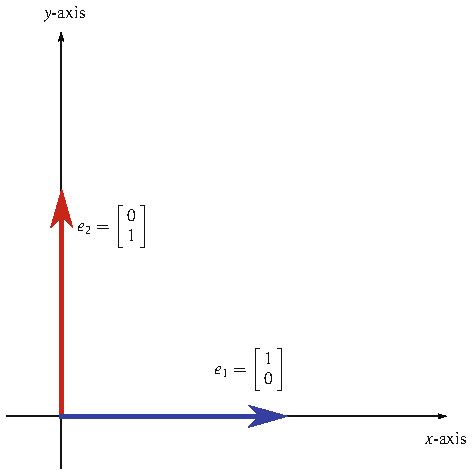
\includegraphics[width=0.561\linewidth]{images/vector/fig-1-1.pdf}
  \caption{笛卡尔平面 $\mathbb{R}^2$，其中显示了向量 $e_1$ 与 $e_2$.}
  \label{fig:1-1}
\end{figure}

\begin{question}\label{q:1-1}
考虑 $\mathbb{R}^2$，其中
\[
u=\begin{bmatrix}u_1\\u_2\end{bmatrix},\quad
v=\begin{bmatrix}v_1\\v_2\end{bmatrix},\quad
w=\begin{bmatrix}w_1\\w_2\end{bmatrix},
\]
且 $c,d\in\mathbb{R}$. 证明 $\mathbb{R}^2$ 的元素满足上述八条公理.
\end{question}

如果你学过线性代数课程，你可能记得向量空间 $V$ 的基是 $V$ 中元素的一个子集 $\beta=\{v_1,\ldots,v_n\}$，它既线性无关又张成向量空间 $V$. 线性无关意味着：如果对某些标量 $a_1,a_2,\ldots,a_n$ 有
\[
a_1v_1+a_2v_2+\cdots+a_nv_n=0,
\]
则必然 $a_1=a_2=\cdots=a_n=0$. 张成意味着：对任意 $v\in V$，都能找到标量 $a_1,a_2,\ldots,a_n$ 使得
\[
v=a_1v_1+a_2v_2+\cdots+a_nv_n.
\]
这不是一门线性代数课程，我们这里的主要目的只是提醒你线性代数中的一些事实，并让你对这些概念有更好的直觉感受，因此不再深入.

欧几里得向量空间 $\mathbb{R}^2$ 是你非常熟悉的空间，它通常被画成如图 \ref{fig:1-1} 那样的笛卡尔平面. 图中显示了两个欧几里得单位向量
\[
e_1=\binom{1}{0},\qquad e_2=\binom{0}{1}.
\]
$\mathbb{R}^2$ 中一个典型向量形如 $\begin{bmatrix}x\\y\end{bmatrix}$，其中 $x,y\in\mathbb{R}$. 容易看出 $e_1$ 与 $e_2$ 线性无关. 假设存在 $a_1$ 与 $a_2$ 使得
\[
a_1\begin{bmatrix}1\\0\end{bmatrix}+a_2\begin{bmatrix}0\\1\end{bmatrix}=\begin{bmatrix}0\\0\end{bmatrix}.
\]
这只能发生在 $a_1=0$ 且 $a_2=0$ 时，这正是为了得出 $e_1$ 与 $e_2$ 线性无关所需证明的. 要看出 $e_1$ 与 $e_2$ 张成 $\mathbb{R}^2$，我们必须证明：对 $\mathbb{R}^2$ 中任意向量 $\begin{bmatrix}x\\y\end{bmatrix}$，都能找到 $a_1$ 与 $a_2$ 使得
\[
\begin{bmatrix}x\\y\end{bmatrix}=a_1\begin{bmatrix}1\\0\end{bmatrix}+a_2\begin{bmatrix}0\\1\end{bmatrix}.
\]
但这显然可以通过令 $a_1=x$、$a_2=y$ 实现. 因此 $e_1$ 与 $e_2$ 张成 $\mathbb{R}^2$，它们被称为标准基向量，有时也称为欧几里得基向量. 显然标准基向量使用起来很方便. 当然，欧几里得单位向量集 $\{e_1,e_2\}$ 并不是 $\mathbb{R}^2$ 唯一可能的基.

\begin{question}\label{q:1-2}
证明向量集
\[
\left\{\begin{bmatrix}2\\0\end{bmatrix},\begin{bmatrix}1\\1\end{bmatrix}\right\}
\]
也是 $\mathbb{R}^2$ 的一组基. 再找出 $\mathbb{R}^2$ 的另一组基.
\end{question}

\begin{question}\label{q:1-3}
现在考虑向量空间 $\mathbb{R}^3$. 这个向量空间通常画成如图 \ref{fig:1-2} 那样. 考虑三个向量
\[
e_1=\begin{bmatrix}1\\0\\0\end{bmatrix},\qquad e_2=\begin{bmatrix}0\\1\\0\end{bmatrix},\qquad e_3=\begin{bmatrix}0\\0\\1\end{bmatrix}.
\]
\begin{enumerate}
  \item[(a)] $\mathbb{R}^3$ 中一个典型向量长什么样？
  \item[(b)] 证明 $e_1,e_2,e_3$ 线性无关.
  \item[(c)] 证明 $e_1,e_2,e_3$ 张成 $\mathbb{R}^3$.
\end{enumerate}
\end{question}

\begin{figure}[htbp]
  \centering
  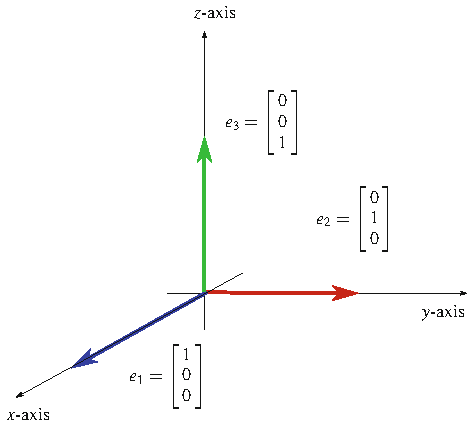
\includegraphics[width=0.562\linewidth]{images/vector/fig-1-2.pdf}
  \caption{笛卡尔空间 $\mathbb{R}^3$，其中显示了向量 $e_1,e_2,e_3$.}
  \label{fig:1-2}
\end{figure}

向量空间 $\mathbb{R}^n$ 是 $n$ 元数组
\[
\begin{bmatrix}x_1\\x_2\\\vdots\\x_n\end{bmatrix}.
\]
对它进行实际的想象是不可能的，但我们通常求助于使用与 $\mathbb{R}^3$ 的图画基本相同的 $\mathbb{R}^n$ 的``漫画式''图画. 欧几里得单位向量
\[
e_1=\begin{bmatrix}1\\0\\\vdots\\0\end{bmatrix},\quad
e_2=\begin{bmatrix}0\\1\\\vdots\\0\end{bmatrix},\quad
e_3=\begin{bmatrix}0\\0\\\vdots\\0\end{bmatrix},\quad\cdots,\quad
e_n=\begin{bmatrix}0\\0\\\vdots\\1\end{bmatrix}
\]
构成向量空间 $\mathbb{R}^n$ 的一组基，称为标准基.

本书中我们将反复做的一件事，就是帮助你建立良好而恰当的图画、漫画和心智图像，以帮助你获得对微分形式及其应用的深入而直观的理解. 有时我们会尝试绘制无法在二维或三维中精确描绘的对象. 在依据这些漫画进行思考时你必须始终小心，其中实际上丢失了大量信息. 然而，我们相信拥有适当的近似图画将大大有助于你理解当前的情形. 最后，我们强调，我们始终把向量空间的元素视为列向量，而从不视为行向量. 其原因到后面就会清楚.

现在我们来考虑向量空间之间的一类特定的变换，称为线性变换，有时也称为线性映射或线性算子. 设 $T$ 是 $\mathbb{R}^n$ 与 $\mathbb{R}^m$ 之间的映射，即 $T:\mathbb{R}^n\to\mathbb{R}^m$. 若 $T$ 具有以下两条性质，则称 $T$ 为线性变换：
\begin{enumerate}
  \item $T(v+w)=T(v)+T(w)$
  \item $T(c\cdot v)=c\cdot T(v)$
\end{enumerate}
其中 $v,w\in\mathbb{R}^n$，$c\in\mathbb{R}$.

第一条性质 $T(v+w)=T(v)+T(w)$ 意味着：对定义域向量空间中两个向量的和施行变换，与先分别对这两个向量施行变换、再在陪域向量空间中对结果求和，得到相同的结果. 第二条性质 $T(c\cdot v)=c\cdot T(v)$ 意味着：对向量的标量倍施行变换，与先对向量施行变换、再将结果乘以标量，得到相同的结果. 若 $T$ 是从 $\mathbb{R}^n$ 到 $\mathbb{R}$ 的线性变换，则它常被简称为线性函数或线性泛函.

我们先考察几个具体的例子. 考虑映射 $T:\mathbb{R}^2\to\mathbb{R}^3$，其定义为
\[
T\binom{x}{y}=\begin{bmatrix}x-y\\x+y\\2x\end{bmatrix}.
\]
首先考虑这个映射对 $\mathbb{R}^2$ 中某个具体元素的作用，
\[
T\binom{4}{10}=\begin{bmatrix}-6\\14\\8\end{bmatrix}.
\]
于是映射 $T$ 把向量 $\binom{4}{10}\in\mathbb{R}^2$ 送到向量 $\begin{bmatrix}-6\\14\\8\end{bmatrix}\in\mathbb{R}^3$. 我们现在的目标是判断映射 $T$ 是否确实是线性变换. 为此我们需要证明两条性质都成立. 从性质一开始，是否有
\[
T\left(\binom{a_1}{a_2}+\binom{b_1}{b_2}\right)=T\binom{a_1}{a_2}+T\binom{b_1}{b_2}?
\]
我们先求出左边的表达式，
\[
T\left(\binom{a_1}{a_2}+\binom{b_1}{b_2}\right)
=T\binom{a_1+b_1}{a_2+b_2}
=\begin{bmatrix}a_1+b_1-a_2-b_2\\a_1+b_1+a_2+b_2\\2a_1+2b_1\end{bmatrix}.
\]
再求出右边的表达式
\[
T\binom{a_1}{a_2}+T\binom{b_1}{b_2}
=\begin{bmatrix}a_1-a_2\\a_1+a_2\\2a_1\end{bmatrix}+\begin{bmatrix}b_1-b_2\\b_1+b_2\\2b_1\end{bmatrix}
=\begin{bmatrix}a_1+b_1-a_2-b_2\\a_1+b_1+a_2+b_2\\2a_1+2b_1\end{bmatrix}.
\]
比较这两个表达式，我们看到性质一确实成立. 接着看性质二，是否有
\[
T\left(c\cdot\binom{a_1}{a_2}\right)=c\cdot T\binom{a_1}{a_2}?
\]
求出左边的表达式，我们有
\[
T\left(c\cdot\binom{a_1}{a_2}\right)
=T\binom{ca_1}{ca_2}
=\begin{bmatrix}ca_1-ca_2\\ca_1+ca_2\\2ca_2\end{bmatrix}.
\]
再求出右边的表达式
\[
c\cdot T\binom{a_1}{a_2}
=c\cdot\begin{bmatrix}a_1-a_2\\a_1+a_2\\2a_2\end{bmatrix}
=\begin{bmatrix}ca_1-ca_2\\ca_1+ca_2\\2ca_2\end{bmatrix}.
\]
比较这两个表达式，我们看到性质二成立. 因此，由于性质一与性质二都成立，映射 $T$ 确实是一个线性变换.

\begin{question}\label{q:1-4}
考虑由
\[
T\binom{x}{y}=\binom{x+y}{y+5}
\]
定义的 $T:\mathbb{R}^2\to\mathbb{R}^2$. $T$ 是线性变换吗？
\end{question}

判断映射 $T:\mathbb{R}^n\to\mathbb{R}$ 是否为线性泛函同样直接. 考虑映射
\[
T\binom{x}{y}=2x+y.
\]
要判断 $T$ 是否为线性泛函，我们同样必须证明性质一与性质二成立. 由于
\[
T\left(\binom{a_1}{a_2}+\binom{b_1}{b_2}\right)=2a_1+2b_1+a_2+b_2
\]
且
\[
T\binom{a_1}{a_2}+T\binom{b_1}{b_2}=2a_1+2b_1+a_2+b_2,
\]
故第一条性质成立. 又由于
\[
T\left(c\cdot\binom{a_1}{a_2}\right)=2ca_1+ca_2
\]
且
\[
c\cdot T\binom{a_1}{a_2}=2ca_1+ca_2,
\]
故第二条性质成立，于是 $T$ 是一个线性泛函.

\begin{question}\label{q:1-5}
考虑下面定义的 $T:\mathbb{R}^2\to\mathbb{R}$. 它们是线性泛函吗？
\begin{enumerate}
  \item[(a)] $T\binom{x}{y}=x^2+y$
  \item[(b)] $T\binom{x}{y}=xy$
  \item[(c)] $T\binom{x}{y}=2x+3y+7$
\end{enumerate}
\end{question}

在把注意力转向线性变换与矩阵之间的关系之前，我们非常简要地回顾一下矩阵与矩阵乘法. 简单地说，矩阵就是一个矩形数表，一般写在方括号内. 例如，
\[
\begin{bmatrix}7&4&-3\\2&-9&5\end{bmatrix},\qquad
\begin{bmatrix}2&-6\\9&4\\11&1\\6&8\end{bmatrix},\qquad
\begin{bmatrix}2&-4&6&7\\-1&8&0&10\\5&2&-3&7\\-2&-4&1&3\end{bmatrix}
\]
都是矩阵的例子. 矩阵的大小用行数和列数表示，通常写作（行数）$\times$（列数）. 例如，上述矩阵的大小分别是 $2\times3$、$4\times2$ 和 $4\times4$. 矩阵中的数有时称为矩阵元素，用带两个下标的变量表示，第一个下标是行号，第二个下标是列号. 这里用一个 $3\times3$ 矩阵展示带下标变量的写法，
\[
\begin{bmatrix}a_{11}&a_{12}&a_{13}\\a_{21}&a_{22}&a_{23}\\a_{31}&a_{32}&a_{33}\end{bmatrix}.
\]
重要的是要记住，行下标在前，列下标在后.

如果你以前从未见过矩阵乘法，它可能看起来有些复杂. 首先，第一个矩阵的列数必须等于第二个矩阵的行数. 其次，乘积矩阵中第 $ij$ 个元素由第一个矩阵的第 $i$ 行与第二个矩阵的第 $j$ 列相乘得到. 在给出一般公式之前，我们先用一个例子说明，
\[
\begin{bmatrix}1&2\\3&4\end{bmatrix}\begin{bmatrix}5&6\\7&8\end{bmatrix}.
\]
乘积矩阵的 $a_{11}$ 项由红色行与蓝色列相乘得到，即
\[
a_{11}=1\cdot5+2\cdot7=19.
\]
类似地，
\begin{align*}
\begin{bmatrix}1&2\\3&4\end{bmatrix}\begin{bmatrix}5&6\\7&8\end{bmatrix}
\Rightarrow a_{12}=1\cdot6+2\cdot8=22, \\
\begin{bmatrix}1&2\\3&4\end{bmatrix}\begin{bmatrix}5&6\\7&8\end{bmatrix}
\Rightarrow a_{21}=3\cdot5+4\cdot7=43, \\
\begin{bmatrix}1&2\\3&4\end{bmatrix}\begin{bmatrix}5&6\\7&8\end{bmatrix}
\Rightarrow a_{22}=3\cdot6+4\cdot8=50.
\end{align*}
把所有这些放在一起，我们得到
\[
\begin{bmatrix}1&2\\3&4\end{bmatrix}\begin{bmatrix}5&6\\7&8\end{bmatrix}
=\begin{bmatrix}19&22\\43&50\end{bmatrix}.
\]

现在我们给出矩阵乘法的一般公式. 若 $A$ 是 $n\times m$ 矩阵，$B$ 是 $m\times p$ 矩阵，
\[
\begin{bmatrix}
a_{11}&a_{12}&\cdots&a_{1m}\\
a_{21}&a_{22}&\cdots&a_{2m}\\
\vdots&\vdots&\ddots&\vdots\\
a_{n1}&a_{n2}&\cdots&a_{nm}
\end{bmatrix}
\begin{bmatrix}
b_{11}&b_{12}&\cdots&b_{1p}\\
b_{21}&b_{22}&\cdots&b_{2p}\\
\vdots&\vdots&\ddots&\vdots\\
b_{m1}&b_{m2}&\cdots&b_{mp}
\end{bmatrix}
=
\begin{bmatrix}
c_{11}&c_{12}&\cdots&c_{1p}\\
c_{21}&c_{22}&\cdots&c_{2p}\\
\vdots&\vdots&\ddots&\vdots\\
c_{n1}&c_{n2}&\cdots&c_{np}
\end{bmatrix},
\]
其中
\[
c_{ij}=\sum_{k=1}^{m}a_{ik}b_{kj}.
\]
注意乘积矩阵的维数是 $n\times p$.

现在我们转向线性变换与矩阵之间的关系. 这不是一门线性代数课程，所以我们不会在向量空间或基上大做文章. 我们只使用向量空间 $\mathbb{R}^n$ 以及由欧几里得单位向量 $e_1,e_2,\ldots,e_n$ 组成的标准基. 严格地说，要把线性变换 $T:\mathbb{R}^n\to\mathbb{R}^m$ 写成矩阵，我们必须为 $\mathbb{R}^n$ 和 $\mathbb{R}^m$ 各取一个有序基；也就是说，基元素必须有一个固定的顺序. 但我们通常认为欧几里得单位向量具有直观上显而易见的顺序，$e_1$ 第一，$e_2$ 第二，$e_3$ 第三，依此类推. 在给出一般定义之前，我们先看几个例子.

考虑我们之前的例子，由
\[
T\binom{x}{y}=\begin{bmatrix}x-y\\x+y\\2x\end{bmatrix}
\]
定义的 $T:\mathbb{R}^2\to\mathbb{R}^3$. 利用线性变换的性质以及矩阵乘法的知识，我们有以下过程
\begin{align*}
T\binom{x}{y}
&=T\left(\binom{x}{0}+\binom{0}{y}\right)\\
&=T\left(x\binom{1}{0}+y\binom{0}{1}\right)\\
&=T\left(x\binom{1}{0}\right)+T\left(y\binom{0}{1}\right) &&\text{性质一}\\
&=xT\binom{1}{0}+yT\binom{0}{1} &&\text{性质二}\\
&=x\begin{bmatrix}1\\1\\2\end{bmatrix}+y\begin{bmatrix}-1\\1\\0\end{bmatrix}\\
&=\begin{bmatrix}1&-1\\1&1\\2&0\end{bmatrix}\binom{x}{y} &&\text{矩阵乘法的定义}
\end{align*}
通过比较左右两端，我们可以看出可以把线性变换 $T$ 写成一个矩阵，即
\[
T\equiv\begin{bmatrix}1&-1\\1&1\\2&0\end{bmatrix}.
\]

这个计算对你来说可能显而易见，你也许会奇怪我们为什么要经历这些步骤. 主要原因是说明答案如何依赖于 $T$ 在 $\mathbb{R}^2$ 的基向量上的作用. 让我们更详细地考虑这一点. 首先让 $T$ 作用在 $\mathbb{R}^2$ 的第一个基向量上，得到
\[
T\binom{1}{0}=\begin{bmatrix}1\\1\\2\end{bmatrix}=1\begin{bmatrix}1\\0\\0\end{bmatrix}+1\begin{bmatrix}0\\1\\0\end{bmatrix}+2\begin{bmatrix}0\\0\\1\end{bmatrix}.
\]
注意 $\mathbb{R}^3$ 的基向量的系数正是 $T$ 的矩阵表示的第一列的各个元素. 类似地，让 $T$ 作用在 $\mathbb{R}^2$ 的第二个基向量上，得到
\[
T\binom{0}{1}=\begin{bmatrix}-1\\1\\0\end{bmatrix}=-1\begin{bmatrix}1\\0\\0\end{bmatrix}+1\begin{bmatrix}0\\1\\0\end{bmatrix}+0\begin{bmatrix}0\\0\\1\end{bmatrix}.
\]
这里 $\mathbb{R}^3$ 的基向量的系数正是 $T$ 的矩阵表示的第二列的各个元素.

现在给出线性变换的矩阵表示的形式定义. 设 $T:\mathbb{R}^n\to\mathbb{R}^m$. 令 $e_1,e_2,\ldots,e_n$ 为 $\mathbb{R}^n$ 的标准基，令 $\tilde{e}_1,\tilde{e}_2,\ldots,\tilde{e}_m$ 为 $\mathbb{R}^m$ 的标准基. 则对 $1\leq j\leq n$，存在唯一的数 $a_{ij}$ 使得
\[
T(e_j)=\sum_{i=1}^{m}a_{ij}\tilde{e}_i.
\]
于是 $T$ 的矩阵表示就是元素为 $a_{ij}$ 的 $m\times n$ 矩阵.

\begin{question}\label{q:1-6}
求线性变换
\[
T\binom{x}{y}=\begin{bmatrix}2x+3y\\0\\2x-5y\end{bmatrix}
\]
的矩阵表示.
\end{question}

现在我们转向线性泛函，它是陪域为 $\mathbb{R}$ 的线性变换这一特例. 考虑之前的线性泛函 $T\binom{x}{y}=2x+y$. 我们求这个线性泛函的矩阵表示，
\[
T\binom{x}{y}=2x+y=[2,1]\binom{x}{y}.
\]
可以看出线性泛函的矩阵表示是 $1\times n$ 矩阵，也就是行向量. 这是重要的一点：线性泛函用行向量表示. 当我们写 $1\times n$ 矩阵（即行向量）时，通常在元素之间加逗号，只是为了使一切清楚.

本节最后一个主要主题是对偶空间的定义. 假设给定一个向量空间 $V$. 在本书中我们考虑的向量空间只有对某个整数 $n$ 的 $\mathbb{R}^n$. $V$ 上所有线性泛函的集合称为 $V$ 的对偶空间，记为 $V^*$.

事实上，$V$ 的对偶空间 $V^*$ 本身也是一个向量空间. 为证明这一点，我们先说明线性泛函的加法意味着什么. 我们可以把两个线性泛函 $S:V\to\mathbb{R}$ 与 $T:V\to\mathbb{R}$ 相加，得到一个新的线性泛函 $S+T:V\to\mathbb{R}$，泛函 $S+T$ 的取值正如你所预期的那样，$(S+T)(v)=S(v)+T(v)$，其中 $v\in V$. 为了证明向量空间 $V$ 的对偶空间 $V^*$（即 $V$ 上线性泛函的集合）本身是一个向量空间，我们必须证明八条向量空间公理都得到满足.

考虑我们写为 $v+w=w+v$ 的第一条公理，其中 $v,w$ 是向量空间的元素. 但现在我们面对的是 $V^*$，其元素为 $S$ 与 $T$. 我们要证明 $S+T=T+S$. 该怎么做呢？我们必须利用线性泛函加法的定义. 对任意元素 $v\in V$，有 $(S+T)(v)=S(v)+T(v)$. 现在回想 $S(v)$ 与 $T(v)$ 都只是实数，而实数加法是交换的，因此 $S(v)+T(v)=T(v)+S(v)$. 最后，利用线性泛函的加法，有 $T(v)+S(v)=(T+S)(v)$. 把这一切放在一起，我们得到 $(S+T)(v)=(T+S)(v)$. 由于这对任意 $v\in V$ 都成立，我们可以写 $S+T=T+S$，从而证明第一条公理得到满足.

\begin{question}\label{q:1-7}
设 $R,S,T:\mathbb{R}^n\to\mathbb{R}$ 是 $V$ 上的线性泛函，即 $R,S,T\in V^*$，且 $c,d$ 是实数. 通过证明其余七条向量空间公理也得到满足，证明 $V^*$ 是一个向量空间.
\end{question}

我们继续考虑具体的向量空间 $\mathbb{R}^2$. 任意元素 $\binom{x}{y}\in\mathbb{R}^2$ 都可以写成
\[
\binom{x}{y}=x\binom{1}{0}+y\binom{0}{1}.
\]
设 $T\in(\mathbb{R}^2)^*$，则
\begin{align*}
T\binom{x}{y}
&=T\left(x\binom{1}{0}+y\binom{0}{1}\right)\\
&=T\left(x\binom{1}{0}\right)+T\left(y\binom{0}{1}\right)\\
&=xT\binom{1}{0}+yT\binom{0}{1}\\
&=xc_1+yc_2
\end{align*}
其中 $c_1=T\binom{1}{0}$、$c_2=T\binom{0}{1}$ 是某些实数. 所以线性泛函 $T\in(\mathbb{R}^2)^*$ 对任意向量 $\binom{x}{y}\in\mathbb{R}^2$ 的作用完全由它在基向量 $\binom{1}{0}$ 与 $\binom{0}{1}$ 上的作用决定. 我们定义两个线性泛函 $T_1$ 与 $T_2$，使它们在这些基向量上的作用如下：
\[
T_1\binom{1}{0}=1,\qquad T_1\binom{0}{1}=0
\]
以及
\[
T_2\binom{1}{0}=0,\qquad T_2\binom{0}{1}=1.
\]

\begin{question}\label{q:1-8}
设 $T_1$ 与 $T_2$ 是上面定义的 $\mathbb{R}^2$ 上的线性泛函.
\begin{enumerate}
  \item[(a)] 证明 $T_1\binom{x}{y}=x$，$T_2\binom{x}{y}=y$.
  \item[(b)] 是否可能把上面的线性泛函 $T$ 写成 $T_1$ 与 $T_2$ 的线性组合？
  \item[(c)] 证明 $\{T_1,T_2\}$ 是 $(\mathbb{R}^2)^*$（即 $\mathbb{R}^2$ 上线性泛函的集合）的一组基.
\end{enumerate}
\end{question}

既然对偶空间是向量空间，那么对偶空间当然有基. 使用欧几里得单位向量的标准记号，
\[
e_1=\binom{1}{0},\qquad e_2=\binom{0}{1},
\]
我们可以写 $T_1(e_1)=1$、$T_2(e_1)=0$、$T_1(e_2)=0$、$T_2(e_2)=1$. 用稍许不同的记号，我们可以把它概括为 $T_i(e_j)=\delta_{ij}$，$i,j=1,2$，其中 $\delta_{ij}$ 称为 \newterm{kronecker-delta}{克罗内克 $\delta$ 函数}{Kronecker delta function}，其定义为
\[
\delta_{ij}=\begin{cases}1&i=j\\0&i\neq j.\end{cases}
\]
由于 $T_i(e_j)=\delta_{ij}$，我们称 $T_1$ 与向量 $e_1$ 对偶，称 $T_2$ 与向量 $e_2$ 对偶，并称 $\{T_1,T_2\}$ 为 $\{e_1,e_2\}$ 的对偶基.

现在引入一点记号，我们常常把 $T_1$ 写成 $e^1$，把 $T_2$ 写成 $e^2$. 注意这里用的是上标而不是下标. 于是我们有 $\{e_1,e_2\}$ 是 $\mathbb{R}^2$ 的标准基，而 $\{e^1,e^2\}$ 是它的对偶基，是对偶空间 $(\mathbb{R}^2)^*$ 的一组基. 我们还常常写 $e^i(e_j)=\delta_j^i$，这与上面定义的克罗内克 $\delta$ 函数完全相同，只是其中一个下标写成上标，以与基元素和对偶基元素上的上下标写法相匹配.

另外，注意 $e^i(e_j)$ 本质上就是函数记号，线性泛函 $e^i$ 以向量 $e_j$ 作为其自变量. 有时这也写作 $\langle e^i,e_j\rangle$.

还回想起我们前面说过，像 $\mathbb{R}^2$ 这样的向量空间的元素总是写成列向量，而微积分课程中通常不采用这一约定，那里的向量常常为了方便写成行向量. 我们在此坚持这一约定的原因是，像 $(\mathbb{R}^2)^*$ 这样的对偶空间的元素总是写成行向量. 由于 $e^1=1\cdot e^1+0\cdot e^2$，我们写 $e^1=[1,0]$. 类似地，由于 $e^2=0\cdot e^1+1\cdot e^2$，我们有 $e^2=[0,1]$. 这使我们能够使用矩阵乘法：
\begin{align*}
e^1(e_1)&=\langle e^1,e_1\rangle=[1,0]\binom{1}{0}=1\\
e^1(e_2)&=\langle e^1,e_2\rangle=[1,0]\binom{0}{1}=0\\
e^2(e_1)&=\langle e^2,e_1\rangle=[0,1]\binom{1}{0}=0\\
e^2(e_2)&=\langle e^2,e_2\rangle=[0,1]\binom{0}{1}=1
\end{align*}
注意这与我们使用克罗内克 $\delta$ 记号得到的结果一致. 正如 $\mathbb{R}^2$ 中任意元素 $v$ 可以写成 $e_1$ 与 $e_2$ 的线性组合并写成列向量，
\[
v=xe_1+ye_2=\binom{x}{y},
\]
$(\mathbb{R}^2)^*$ 中任意元素 $\alpha$ 也可以写成 $e^1$ 与 $e^2$ 的线性组合并写成行向量
\[
\alpha=ae^1+be^2=[a,b].
\]
于是我们可以用矩阵乘法求出
\[
\alpha(v)=\langle\alpha,v\rangle=[a,b]\binom{x}{y}=ax+by.
\]

所有这些当然可以推广到任意向量空间 $V$，而且你会经常（虽然不是总是）看到 $V$ 的基元素用下标书写，$V^*$ 的基元素用上标书写. 例如，若 $\{v_1,v_2,\ldots,v_n\}$ 是某个向量空间 $V$ 的基，则我们把它在 $V^*$ 中的对偶基写为 $\{v^1,v^2,\ldots,v^n\}$. 于是任意 $v\in V$ 都可以写成 $\{v_1,v_2,\ldots,v_n\}$ 的线性组合，从而写成列向量；任意 $\alpha\in V^*$ 都可以写成 $\{v^1,v^2,\ldots,v^n\}$ 的线性组合，从而写成行向量. 这使得 $\alpha(v)$ 可以通过矩阵乘法计算，即行向量乘以列向量. 这也解释了为什么我们总是把向量空间的元素写成列向量：因为对偶空间的元素写成行向量，而始终区分向量空间元素与对偶空间元素非常重要. 在向量微积分课程中不引入对偶空间，因此为了方便，向量有时写成行向量. 我们在本书中绝不这样做.

\begin{question}\label{q:1-9}
考虑带标准欧几里得基
\[
e_1=\begin{bmatrix}1\\0\\0\end{bmatrix},\qquad e_2=\begin{bmatrix}0\\1\\0\end{bmatrix},\qquad e_3=\begin{bmatrix}0\\0\\1\end{bmatrix}
\]
的向量空间 $\mathbb{R}^3$. 令
\[
v=\begin{bmatrix}x\\y\\z\end{bmatrix}=xe_1+ye_2+ze_3\in\mathbb{R}^3.
\]
设 $(\mathbb{R}^3)^*$ 为 $\mathbb{R}^3$ 的对偶空间，其对偶基为
\[
e^1=[1,0,0],\qquad e^2=[0,1,0],\qquad e^3=[0,0,1].
\]
现在考虑线性泛函
\[
f\begin{pmatrix}\begin{bmatrix}x\\y\\z\end{bmatrix}\end{pmatrix}=3x+2y-6z.
\]
\begin{enumerate}
  \item[(a)] 验证 $f$ 确实是一个线性泛函.
  \item[(b)] 令 $v=\begin{bmatrix}-3\\4\\7\end{bmatrix}$. 求 $f(v)$.
  \item[(c)] 对 $i=1,2,3$ 求 $f(e_i)$.
  \item[(d)] 把 $f$ 写成 $e^1,e^2,e^3$ 的线性组合.
  \item[(e)] 把 $f\in(\mathbb{R}^3)^*$ 写成行向量.
  \item[(f)] 用矩阵乘法写出 $f(v)$.（即行向量 $f$ 乘以列向量 $v$.）
\end{enumerate}
\end{question}

\begin{question}\label{q:1-10}
考虑带标准欧几里得基 $e_1,e_2,e_3,e_4$ 的向量空间 $\mathbb{R}^4$，以及带标准对偶基 $e^1,e^2,e^3,e^4$ 的对偶空间 $(\mathbb{R}^4)^*$. 令
\[
v=\begin{bmatrix}x_1\\x_2\\x_3\\x_4\end{bmatrix}\in\mathbb{R}^4,
\]
并定义线性泛函 $f$ 为 $f(v)=5x_1-2x_2+7x_3-6x_4$.
\begin{enumerate}
  \item[(a)] 验证 $f\in(\mathbb{R}^4)^*$.（即 $f$ 是一个线性泛函.）
  \item[(b)] 对 $i=1,2,3,4$ 求 $f(e_i)$，并据此把 $f$ 写成行向量.
  \item[(c)] 用表示 $f$ 的行向量求
  \[
  f\begin{pmatrix}\begin{bmatrix}-7\\3\\2\\-1\end{bmatrix}\end{pmatrix}
  \qquad\text{与}\qquad
  f\begin{pmatrix}\begin{bmatrix}1/2\\-4\\-2/3\\5\end{bmatrix}\end{pmatrix}.
  \]
\end{enumerate}
\end{question}

让我们更仔细地看看对偶基元素. 以 $(\mathbb{R}^4)^*$ 为例，我们考虑对偶基元素 $e^1,e^2,e^3,e^4$. 考虑 $\mathbb{R}^4$ 中的如下向量，
\[
v=\begin{bmatrix}2\\-5\\7\\-9\end{bmatrix}.
\]
让我们看看对偶基元素如何作用于 $v$. 我们有
\[
e^1(v)=[1,0,0,0]\begin{bmatrix}2\\-5\\7\\-9\end{bmatrix}=2.
\]
类似地，有 $e^2(v)=-5$、$e^3(v)=7$、$e^4(v)=-9$. 可以看出，本质上对偶基元素``挑出''相应的向量坐标：$e^1$ 挑出第一个坐标，$e^2$ 挑出第二个坐标，$e^3$ 挑出第三个坐标，$e^4$ 挑出第四个坐标.

现在我们将探讨常被用来描绘线性泛函的漫画之一. 我们有意使用``漫画''这个词. 我们所建立的是一些不完美的心智图像，以便尝试想象正在发生的事情. 重要的是要记住这些图像并不精确，然而它们使我们能够发展对数学概念的直觉. 根据我们的经验，我们将在这里开始建立的这种漫画表示在物理学中最常见. 我们用 $\mathbb{R}^2$ 和 $(\mathbb{R}^2)^*$ 作为示例空间开始.

令
\[
e_1=\binom{1}{0},\qquad e_2=\binom{0}{1}
\]
为向量空间 $\mathbb{R}^2$ 的一组基. 这组基诱导出 $(\mathbb{R}^2)^*$ 的对偶基 $e^1=[1,0]$ 与 $e^2=[0,1]$. 考虑 $\mathbb{R}^2$ 中的如下向量：
\[
\binom{1}{3},\ \binom{1}{2},\ \binom{1}{1},\ \binom{1}{0},\ \binom{1}{-1},\ \binom{1}{-2},\ \binom{1}{-3}.
\]
显然 $e^1$ 作用于这些向量中的每一个都给出 $1$. 现在考虑向量：
\[
\binom{2}{3},\ \binom{2}{2},\ \binom{2}{1},\ \binom{2}{0},\ \binom{2}{-1},\ \binom{2}{-2},\ \binom{2}{-3}.
\]
我们有 $e^1$ 把所有这些向量送到 $2$. 以同样的方式，$e^1$ 把任意形如 $\binom{0}{y}$（其中 $y\in\mathbb{R}$）的向量送到 $0$. 它把任意形如 $\binom{-1}{y}$ 的向量送到 $-1$，依此类推. 如图 \ref{fig:1-3} 那样画出这些向量，可以看出：$e^1$ 送到 $1$ 的那些向量的终点位于竖直线 $x=1$ 上，$e^1$ 送到 $2$ 的那些向量的终点位于竖直线 $x=2$ 上，$e^1$ 送到 $0$ 的那些向量的终点位于竖直线 $x=0$ 上，$e^1$ 送到 $-1$ 的那些向量的终点位于竖直线 $x=-1$ 上，依此类推. 这给出了一种构造线性泛函 $e^1$ 的漫画图像的方法，即在向量空间 $\mathbb{R}^2$ 上画出整数水平集，如图 \ref{fig:1-4} 所示. 考虑图中所示的向量，
\[
A=\binom{3.5}{1.5},\qquad B=\binom{-3.5}{1.5},\qquad C=\binom{1.9}{-1},\qquad D=\binom{-1.5}{-1.5},
\]
显然 $e^1(A)=3.5$、$e^1(B)=-3.5$、$e^1(C)=1.9$、$e^1(D)=-1.5$.

\begin{figure}[htbp]
  \centering
  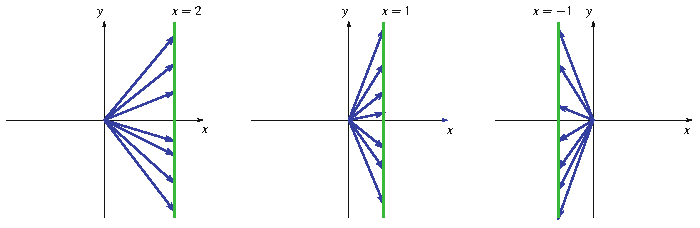
\includegraphics[width=0.960\linewidth]{images/vector/fig-1-3.pdf}
  \caption{终点的 $x$ 值分别为 $2$、$1$、$-1$ 的向量草图}
  \label{fig:1-3}
\end{figure}

\begin{figure}[htbp]
  \centering
  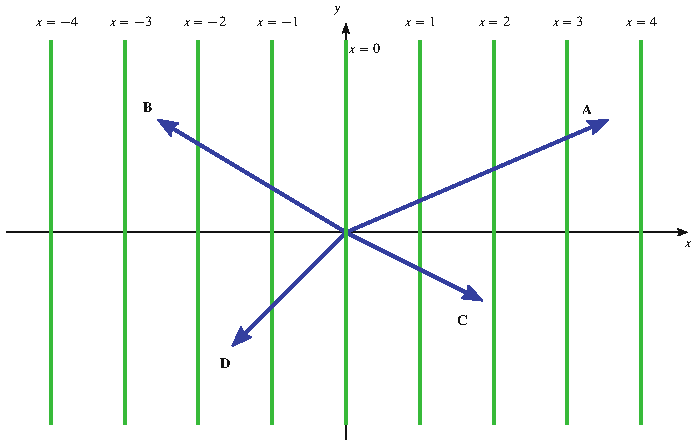
\includegraphics[width=0.915\linewidth]{images/vector/fig-1-4.pdf}
  \caption{向量空间 $\mathbb{R}^2$ 上描绘线性泛函 $e^1$ 的``水平集''，以及向量 $A,B,C,D$}
  \label{fig:1-4}
\end{figure}

使用 $e^1$ 的这幅漫画图像只能给出近似答案，但它提供了一种很好的方式来可视化和理解 $e^1$ 的作用. 有时在物理学中你会听到这样的说法：线性泛函所给出的``向量的值''，等于该向量刺穿的该线性泛函的水平集的个数. 本质上，线性泛函 $e^1$ 的这幅图像通过数向量``刺穿''或穿过的竖直水平集的个数来起作用，同时仍然记录符号. 也就是说，我们把负的水平集计为负的. 如果向量的终点落在一个水平集上，则该水平集被视为被``刺穿''，并计入总数. 例如，在图 \ref{fig:1-4} 中，向量 $A$ 刺穿 3 个水平集，向量 $C$ 刺穿 1 个水平集，而向量 $B$ 刺穿 $-3$ 个水平集，向量 $D$ 刺穿 $-1$ 个水平集. 因此，根据我们的漫画图像，有 $e^1(A)=3$、$e^1(B)=-3$、$e^1(C)=1$、$e^1(D)=-1$，这与实际值很接近. 类似的分析得到 $e^2$ 如图 \ref{fig:1-5} 所示.

\begin{question}\label{q:1-11}
考虑线性泛函 $e^2\in(\mathbb{R}^2)^*$.
\begin{enumerate}
  \item[(a)] 给出 $e^2$ 送到 $1$、$2$、$0$、$-1$ 的五个向量.
  \item[(b)] 画出这些向量，并用它们的终点画出水平集.
\end{enumerate}
\end{question}

\begin{figure}[htbp]
  \centering
  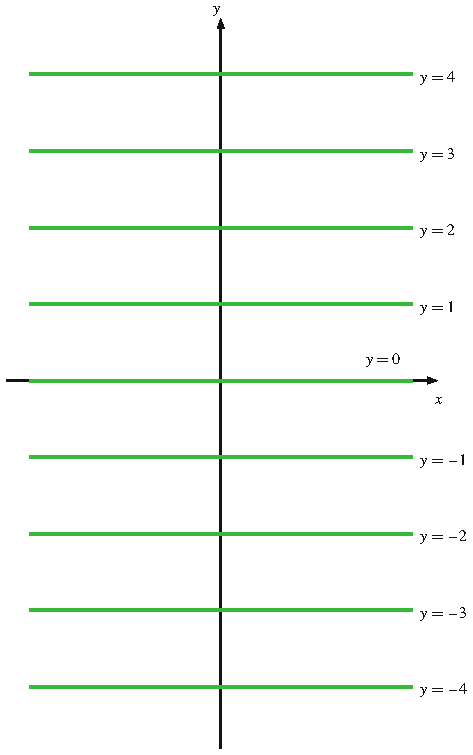
\includegraphics[width=0.561\linewidth]{images/vector/fig-1-5.pdf}
  \caption{向量空间 $\mathbb{R}^2$ 上描绘线性泛函 $e^2$ 的``水平集''}
  \label{fig:1-5}
\end{figure}

想一想 $e^1$ 与 $e^2$ 的两幅漫画. $xy$ 坐标轴代表向量空间 $\mathbb{R}^2$. 然而 $e^1$ 与 $e^2$ 实际上位于对偶空间 $(\mathbb{R}^2)^*$ 中. 在某种意义上我们做的事情很奇怪，我们试图在 $\mathbb{R}^2$ 中画出 $e^1$ 与 $e^2$ 的图像，而它们是 $(\mathbb{R}^2)^*$ 的元素. 考虑我们在 $\mathbb{R}^2$ 中画的 $e^1$ 的图与图 \ref{fig:1-6} 中我们在 $(\mathbb{R}^2)^*$ 中画的 $e^1$ 的图有多么不同. 类似地，我们在 \ref{fig:1-7} 中画出 $e^2$ 在 $\mathbb{R}^2$ 中的图与 $e^2$ 在 $(\mathbb{R}^2)^*$ 中的图.

\begin{figure}[htbp]
  \centering
  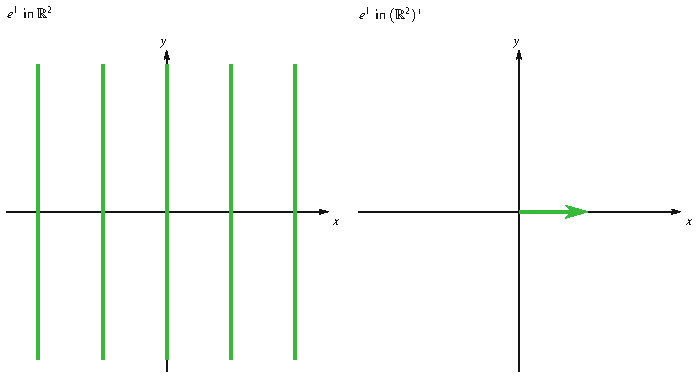
\includegraphics[width=0.929\linewidth]{images/vector/fig-1-6.pdf}
  \caption{描绘线性泛函 $e^1$ 的水平集：画在向量空间 $\mathbb{R}^2$ 上（左），以及把线性泛函 $e^1$ 画成向量空间 $(\mathbb{R}^2)^*$ 中的向量（右）}
  \label{fig:1-6}
\end{figure}

\begin{figure}[htbp]
  \centering
  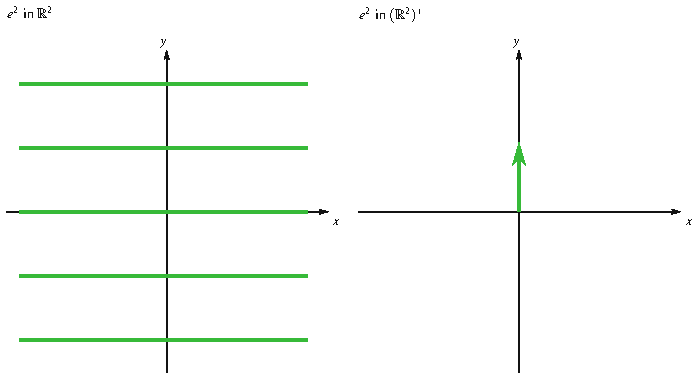
\includegraphics[width=0.929\linewidth]{images/vector/fig-1-7.pdf}
  \caption{描绘线性泛函 $e^2$ 的水平集：画在向量空间 $\mathbb{R}^2$ 上（左），以及把线性泛函 $e^2$ 画成向量空间 $(\mathbb{R}^2)^*$ 中的向量（右）}
  \label{fig:1-7}
\end{figure}

现在我们来看一个稍复杂的线性泛函 $f=2e^1+e^2\in(\mathbb{R}^2)^*$. 首先问自己：$f$ 把哪些向量 $v$ 送到 $1$？即求满足 $f(v)=1$ 的 $v$：
\begin{align*}
1=f\binom{x}{y}=2e^1\binom{x}{y}+e^2\binom{x}{y}=2x+y \\
\Rightarrow\quad 2x+y=1\quad\Rightarrow\quad y=-2x+1.
\end{align*}
换句话说，$\Rightarrow f\binom{x}{-2x+1}=1$，其中 $x$ 是任意实数. 我们还发现，线性泛函 $f$ 送到 $1$ 的那些向量 $v$ 的终点确定直线 $y=-2x+1$. 因此我们的 $1$ 的水平集由方程 $y=-2x+1$ 给出.

\begin{question}\label{q:1-12}
求 $f$ 送到 $2$、$3$、$0$、$-1$、$-2$ 的向量. 用这些向量确定这些值对应的水平集.
\end{question}

把我们在问题中找到的 $f$ 的水平集画出来，就得到 $f$ 在 $\mathbb{R}^2$ 上的图像，如图 \ref{fig:1-8} 所示. 考虑图中所示的两个向量，
\[
A=\binom{1/2}{1},\qquad B=\binom{1}{-3}.
\]

\begin{figure}[htbp]
  \centering
  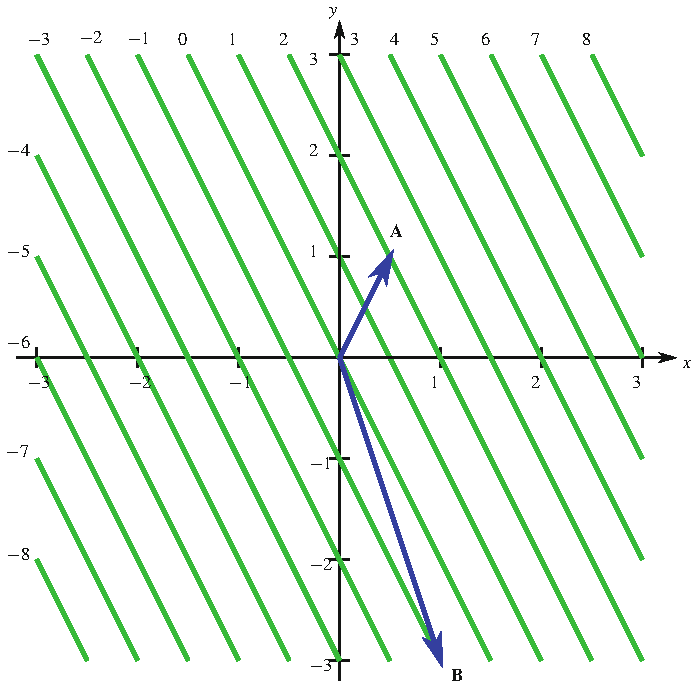
\includegraphics[width=0.826\linewidth]{images/vector/fig-1-8.pdf}
  \caption{向量空间 $\mathbb{R}^2$ 上描绘线性泛函 $f=2e^1+e^2$ 的水平集，以及向量 $A$ 与 $B$}
  \label{fig:1-8}
\end{figure}

显然 $A$ 刺穿两个水平集，因此根据我们的图像 $f(A)=2$；而 $B$ 刺穿 $-1$ 个水平集，因此根据我们的图像 $f(B)=-1$. 用计算来复核我们的图像，我们有
\begin{align*}
f(A)=2e^1(A)+e^2(A)=2\cdot\frac12+1=2 \\
f(B)=2e^1(B)+e^2(B)=2(1)-3=-1,
\end{align*}
这正是我们所预期的. 线性泛函的漫画图像可以很容易地推广到 $\mathbb{R}^3$. 我们这里不这样做，但我们将在后面的一章中在稍许不同的背景下考虑这种情况.

\section{体积与行列式}

矩阵的行列式具有广泛的性质和用途. 然而，对我们来说，行列式最有用的地方在于它与体积的联系：矩阵的行列式给出由矩阵各列给出的向量所张成的平行六面体的有向体积. 它与我们对体积的直观概念的唯一区别在于，这里的体积带有正号或负号. 因此，虽然我们习惯于认为体积是正的（或零），但事实上它也可以是负的. 而如果说这还不够奇怪的话，真正离奇的是，我们对体积应有行为的直觉观念恰恰迫使我们接受这个符号.

行列式有各种各样的引入方式，坦白说，其中许多方式一点也不清楚. 由于真正理解行列式与体积的关系对我们很重要，我们将实际利用对体积的直观理解以及我们期望体积具有的三条性质来推导行列式. 令人惊叹的是，体积应有行为的这三条性质唯一地确定了行列式.

那么，我们期望体积如何表现？首先，我们期望单位立方体（就这件事而言，单位 $n$ 立方体）的体积为 1. 这源于 $1^3$（或 $1^n$）等于 1 这一事实. 这实际上对我们的体积进行了归一化. 其次，我们期望退化平行六面体的体积为零. 基本上，在 $n$ 维空间中，任何 $n-1$ 维对象的 $n$ 维体积都是零. 例如，$\mathbb{R}^3$ 中的一个二维单位正方形具有零三维体积，即使在 $\mathbb{R}^2$ 中它的二维体积为 1. 第三，我们期望体积是线性的. 线性意味着几件事，其中之一是：如果固定 $n$ 维平行六面体的 $n-1$ 条边，并把剩下的一条边按某个因子缩放，那么平行六面体的体积也按该因子改变. 所以，如果我们把 3 立方体一条边的长度加倍，那么体积也将加倍. 现在，带着这些一般想法，让我们进入实际的数学.

假设我们有一个平行六面体 $P\in\mathbb{R}^n$，其边由 $v_1,v_2,\ldots,v_n\in\mathbb{R}^n$ 给出. 我们说平行六面体 $P$ 是向量 $v_1,v_2,\ldots,v_n$ 的张成，并写 $P=\mathrm{span}\{v_1,v_2,\ldots,v_n\}$. 注意这里``张成''一词的用法与上一节不同，上一节我们说向量空间的基张成该向量空间. 我们想找一个函数 $D:\mathbb{R}^{n\times n}\to\mathbb{R}$，它把 $v_1,v_2,\ldots,v_n$（或者类似地，以 $v_1,v_2,\ldots,v_n$ 为列的矩阵 $M$）送到一个实数，即 $P$ 的体积. 让记号灵活一些，我们既可以写 $D(M)$，也可以写 $D(v_1,v_2,\ldots,v_n)$. 现在，我们用数学的严谨性来表述体积的三条直观性质.

\begin{property}{1}\label{prop:1-1}
$D(I)=1$，其中 $I=[e_1,e_2,\ldots,e_n]$，即单位矩阵.
\end{property}

这说的是单位 $n$ 立方体的体积为 1. 二维和三维的例子如图 \ref{fig:1-9} 所示. 注意单位 $n$ 立方体由 $\mathrm{span}\{e_1,e_2,\ldots,e_n\}$ 给出，而单位矩阵 $I$ 由 $I=[e_1,e_2,\ldots,e_n]$ 给出. 因此我们也常常用 $I$ 来记单位 $n$ 立方体.

\begin{figure}[htbp]
  \centering
  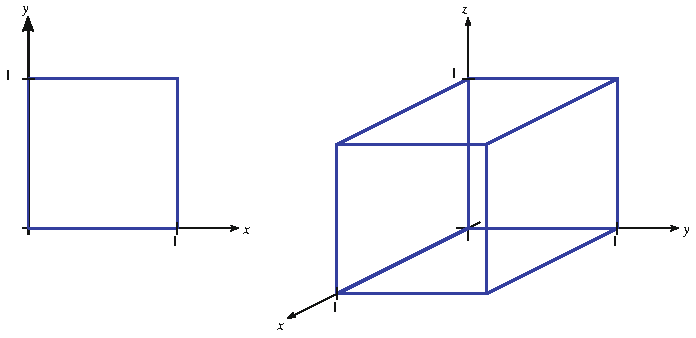
\includegraphics[width=0.856\linewidth]{images/vector/fig-1-9.pdf}
  \caption{单位正方形的二维体积（即面积）为 $1$（左），单位立方体的三维体积也为 $1$（右）}
  \label{fig:1-9}
\end{figure}

\begin{property}{2}\label{prop:1-2}
若对任意 $i\neq j$ 有 $v_i=v_j$，则 $D(v_1,v_2,\ldots,v_n)=0$.
\end{property}

这条性质说的是，如果 $n$ 平行六面体的任意两条边相同，也就是说，如果平行六面体是退化的，那么体积为零. 图 \ref{fig:1-10} 在三维空间中的二维平行六面体上展示了这一点.

\begin{figure}[htbp]
  \centering
  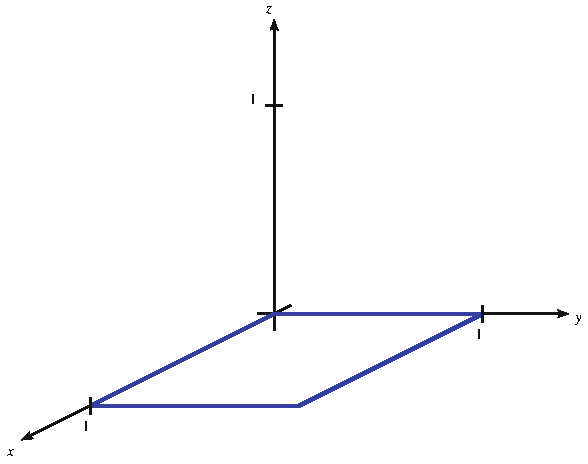
\includegraphics[width=0.721\linewidth]{images/vector/fig-1-10.pdf}
  \caption{三维空间中二维平行六面体的三维体积为零}
  \label{fig:1-10}
\end{figure}

\begin{property}{3}\label{prop:1-3}
$D$ 是线性的. 即，对任意 $j=1,\ldots,n$，
\begin{align*}
D(v_1,\ldots,v_{j-1},v+cw,v_{j+1},\ldots,v_n)
&=D(v_1,\ldots,v_{j-1},v,v_{j+1},\ldots,v_n)\\
&\quad+c\,D(v_1,\ldots,v_{j-1},w,v_{j+1},\ldots,v_n).
\end{align*}
\end{property}

实际上，这说的比``如果我们把一条边的长度按因子缩放，体积也按该因子缩放''稍多一点. 这条性质还包括剪切，但由欧几里得几何我们知道剪切也不改变体积. 图 \ref{fig:1-11} 对二维平行六面体展示了缩放.

\begin{figure}[htbp]
  \centering
  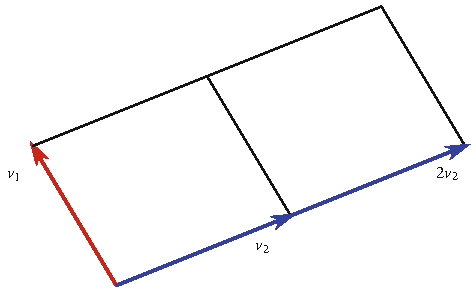
\includegraphics[width=0.564\linewidth]{images/vector/fig-1-11.pdf}
  \caption{把此二维平行六面体一条边的长度加倍，二维体积也加倍}
  \label{fig:1-11}
\end{figure}

我们将用体积的这三条性质来推导一个用 $M=[v_1,v_2,\ldots,v_n]$ 的元素表示 $D$ 的具体公式. 通过推导 $D$ 的具体公式，我们也就证明了 $D$ 既存在又唯一. 当然，$D$ 的这个公式就是你所熟知并喜爱、或者可能深恶痛绝的矩阵行列式公式. 遗憾的是，无法回避的事实是，这个公式既丑得吓人，计算起来又实在麻烦. 但生活（和数学）有时就是这样.

我们首先利用上面的三条性质来确定推导 $D$ 的公式所必需的另外几条性质. 我们要证明的第一件事是那个令人惊讶的事实：体积是带符号的.

\begin{property}{A}\label{prop:1-A}
$D$ 是交替的，即若交换任意两个向量，符号改变：
\[
D(v_1,\ldots,v_i,\ldots,v_j,\ldots,v_n)=-D(v_1,\ldots,v_j,\ldots,v_i,\ldots,v_n).
\]
\end{property}

\begin{proof}
为了使记号简单，我们本可以简单地把它写成 $D(v_i,v_j)=-D(v_j,v_i)$，因为 $v_i$ 与 $v_j$ 是我们关心的仅有的两个向量，其余的保持不变. 下面我们使用这个简化的记号.
\begin{align*}
D(v_i,v_j)&=D(v_i,v_j)+D(v_i,v_i) &&\text{性质 2}\\
&=D(v_i,v_j+v_i) &&\text{性质 3}\\
&=D(v_i,v_j+v_i)-D(v_j+v_i,v_j+v_i) &&\text{性质 2}\\
&=D(-v_j,v_j+v_i) &&\text{性质 3}\\
&=-D(v_j,v_j+v_i) &&\text{性质 3}\\
&=-D(v_j,v_j)-D(v_j,v_i) &&\text{性质 3}\\
&=-D(v_j,v_i) &&\text{性质 2}
\end{align*}
\end{proof}

\begin{property}{B}\label{prop:1-B}
若向量 $v_1,v_2,\ldots,v_n$ 线性相关，则
\[
D(v_1,v_2,\ldots,v_n)=0.
\]
\end{property}

\begin{proof}
由线性相关向量的定义，至少有一个向量可以写成其余向量的线性组合. 不失一般性，假设我们可以写 $v_1=c_2v_2+\cdots+c_nv_n$，其中 $c_i$ 是标量. 反复使用性质 3，我们有
\begin{align*}
D(v_1,v_2,\ldots,v_n)
&=D(c_2v_2+\cdots+c_nv_n,v_2,\ldots,v_n)\\
&=c_2D(v_2,v_2,\ldots,v_n)+c_3D(v_3,v_2,\ldots,v_n)+\cdots+c_nD(v_n,v_2,\ldots,v_n)\\
&=0
\end{align*}
其中最后一个等号来自反复使用性质 2.
\end{proof}

在上面的证明中，``不失一般性''这个短语是什么意思？注意我们假设可以把第一个向量 $v_1$ 写成其余向量的线性组合. 尽管我们在证明中针对 $v_1=c_2v_2+\cdots+c_nv_n$ 这个具体例子做了计算，但如果我们改变假设，决定改为 $v_i=c_1v_1+\cdots+c_{i-1}v_{i-1}+c_{i+1}v_{i+1}+\cdots+c_nv_n$ 对任意 $v_i$ 成立，那么计算将本质相同并给出相同的结果. 当然，我们不会把本质上相同的计算重复 $n$ 遍，那将浪费时间和精力. 数学家的绕行办法是使用``不失一般性''这个短语，然后只对一种具体情况做计算. 大家理解，如果你真的愿意去执行计算，所有其他情况都将完全相同并给出相同的结果.

\begin{property}{C}\label{prop:1-C}
把一个向量的倍数加到另一个向量上不改变行列式.
\end{property}

\begin{proof}
不失一般性，假设我们把 $c$ 倍的 $v_j$ 加到 $v_i$ 上.
\begin{align*}
D(v_1,\ldots,v_i+cv_j,\ldots,v_n)
&=D(v_1,\ldots,v_i,\ldots,v_n)+cD(v_1,\ldots,v_j,\ldots,v_n)\\
&=D(v_1,\ldots,v_i,\ldots,v_n)
\end{align*}
其中最后一个等号来自性质 2，因为向量 $v_j$ 重复出现.
\end{proof}

\begin{question}\label{q:1-13}
解释在性质 C 的证明中``不失一般性''这个短语是如何使用的.
\end{question}

有了这些性质，我们几乎准备好推导行列式的公式了. 为此所需的最后一个要素是置换. 因此我们花一点时间回顾置换. 集合 $\{1,\ldots,n\}$ 的置换是从 $\{1,\ldots,n\}$ 到自身的双射（一一且映上）函数. $\{1,\ldots,n\}$ 的置换集合通常记为 $S_n$. 于是 $S_n$ 的每个元素实际上都是一个置换函数，而 $S_n$ 中有 $n!$ 个元素.

\begin{question}\label{q:1-14}
解释在置换函数的语境中一一与映上是什么意思.
\end{question}

看出 $S_n$ 中有 $n!$ 个元素是相当直接的. 设 $\sigma\in S_n$. 则 $\sigma:\{1,\ldots,n\}\to\{1,\ldots,n\}$. 因此 $\sigma(1)$ 有 $n$ 种可能的选择，即 $\{1,\ldots,n\}$ 中的任意元素. $\sigma(2)$ 可以是 $\{1,\ldots,n\}$ 中除 $\sigma(1)$ 之外的任意元素，因为 $\sigma$ 是一一的，所以它有 $n-1$ 种可能的选择. 类似地，$\sigma(3)$ 可以是 $\{1,\ldots,n\}$ 中除 $\sigma(1)$ 或 $\sigma(2)$ 之外的任意元素，所以有 $n-2$ 种可能的选择. 这样继续下去，直到 $\sigma(n)$ 由剩下的那个元素决定. 总之，$\{1,\ldots,n\}$ 的置换总数为
\[
n\cdot(n-1)\cdot(n-2)\cdot\cdots\cdot1=n!.
\]

我们把一个具体的置换 $\sigma$ 记为
\[
\begin{pmatrix}1&2&\cdots&n\\\downarrow&\downarrow&\cdots&\downarrow\\\sigma(1)&\sigma(2)&\cdots&\sigma(n)\end{pmatrix}.
\]
这种记号称为 Cauchy 两行记号，虽然清楚，但也很笨拙. 只取这个数组的第二行，就得到更简洁的 Cauchy 单行记号，即有序列表 $\bigl(\sigma(1),\sigma(2),\ldots,\sigma(n)\bigr)$. 因此，若 $\sigma\in S_3$，我们写 $(2,1,3)$ 表示
\[
\begin{pmatrix}1&2&3\\\downarrow&\downarrow&\downarrow\\2&1&3\end{pmatrix}.
\]
注意，有些书使用循环记号，其中 $(2,1,3)$ 表示
\[
\begin{pmatrix}1&2&3\\\downarrow&\downarrow&\downarrow\\3&1&2\end{pmatrix}.
\]
也就是说，列表的第一个元素被映到第二个，第二个被映到第三个，最后一个被映到第一个，$2\mapsto1\mapsto3\mapsto2$. 在查阅其他书时要小心，务必弄清它们使用哪种记号. 在循环记号中，上面的 $\sigma$ 可以简单地写为 $(1,2)$，其中把自身映到自身的固定元素 3 不写出来. 然而，在这里我们只使用 Cauchy 单行记号或两行记号.

只交换两个元素的置换称为对换. 我们使用对换的特殊记号：$\tau_{i,j}$ 表示 $i$ 与 $j$ 交换，所有其他元素固定. 我们用一个希望能使想法清楚的例子来说明：对换 $\tau_{3,7}\in S_8$ 由
\[
\begin{pmatrix}1&2&3&4&5&6&7&8\\\downarrow&\downarrow&\downarrow&\downarrow&\downarrow&\downarrow&\downarrow&\downarrow\\1&2&7&4&5&6&3&8\end{pmatrix}
\]
给出.

接下来我们注意到，两个置换的复合仍然是一个置换. 为了这个例子的目的，我们使用 $S_5$，它足够大而不平凡，又足够小而易于处理. 设 $\sigma\in S_5$ 由
\[
\begin{pmatrix}1&2&3&4&5\\\downarrow&\downarrow&\downarrow&\downarrow&\downarrow\\4&3&1&5&2\end{pmatrix}
\]
给出，对换 $\tau_{1,3}\in S_5$ 由
\[
\begin{pmatrix}1&2&3&4&5\\\downarrow&\downarrow&\downarrow&\downarrow&\downarrow\\3&2&1&4&5\end{pmatrix}
\]
给出. 我们把复合 $\tau_{1,3}\circ\sigma$ 写为
\[
\begin{array}{c c c c c c}
\sigma&1&2&3&4&5\\
\downarrow&\downarrow&\downarrow&\downarrow&\downarrow&\downarrow\\
&4&3&1&5&2\\
\tau_{1,3}&\downarrow&\downarrow&\downarrow&\downarrow&\downarrow\\
&4&1&3&5&2
\end{array}
\]
注意由于中间一行不是按升序排列的，这并不完全是 Cauchy 两行记号，但所发生的事应该很清楚. 对换 $\tau_{1,3}$ 用红色标出，以帮助阅读这个图示. 其次，不难看出，可以找到一串对换把任意给定的置换变成恒等置换. 例如，置换 $\tau_{3,4}\circ\tau_{2,4}\circ\tau_{2,3}\circ\tau_{2,5}\circ\tau_{1,4}\circ\tau_{1,3}\circ\sigma$ 是恒等置换：
\[
\begin{array}{c c c c c c}
\sigma&1&2&3&4&5\\
\downarrow&\downarrow&\downarrow&\downarrow&\downarrow&\downarrow\\
&4&3&1&5&2\\
\tau_{1,3}&\downarrow&\downarrow&\downarrow&\downarrow&\downarrow\\
&4&1&3&5&2\\
\tau_{1,4}&\downarrow&\downarrow&\downarrow&\downarrow&\downarrow\\
&1&4&3&5&2\\
\tau_{2,5}&\downarrow&\downarrow&\downarrow&\downarrow&\downarrow\\
&1&4&3&2&5\\
\tau_{2,3}&\downarrow&\downarrow&\downarrow&\downarrow&\downarrow\\
&1&4&2&3&5\\
\tau_{2,4}&\downarrow&\downarrow&\downarrow&\downarrow&\downarrow\\
&1&2&4&3&5\\
\tau_{3,4}&\downarrow&\downarrow&\downarrow&\downarrow&\downarrow\\
&1&2&3&4&5
\end{array}
\]
但注意 $\tau_{4,5}\circ\tau_{3,4}\circ\tau_{2,3}\circ\tau_{1,4}\circ\sigma$，
\[
\begin{array}{c c c c c c}
\sigma&1&2&3&4&5\\
\downarrow&\downarrow&\downarrow&\downarrow&\downarrow&\downarrow\\
&4&3&1&5&2\\
\tau_{1,4}&\downarrow&\downarrow&\downarrow&\downarrow&\downarrow\\
&1&3&4&5&2\\
\tau_{2,3}&\downarrow&\downarrow&\downarrow&\downarrow&\downarrow\\
&1&2&4&5&3\\
\tau_{3,4}&\downarrow&\downarrow&\downarrow&\downarrow&\downarrow\\
&1&2&3&5&4\\
\tau_{4,5}&\downarrow&\downarrow&\downarrow&\downarrow&\downarrow\\
&1&2&3&4&5
\end{array}
\]
也给出恒等置换. $\tau_{2,3}\circ\tau_{1,3}\circ\tau_{4,5}\circ\tau_{2,5}\circ\tau_{2,4}\circ\tau_{4,5}\circ\tau_{1,4}\circ\tau_{2,4}\circ\sigma$ 也是如此，
\[
\begin{array}{c c c c c c}
\sigma&1&2&3&4&5\\
\downarrow&\downarrow&\downarrow&\downarrow&\downarrow&\downarrow\\
&4&3&1&5&2\\
\tau_{3,4}&\downarrow&\downarrow&\downarrow&\downarrow&\downarrow\\
&3&4&1&5&2\\
\tau_{1,4}&\downarrow&\downarrow&\downarrow&\downarrow&\downarrow\\
&3&1&4&5&2\\
\tau_{4,5}&\downarrow&\downarrow&\downarrow&\downarrow&\downarrow\\
&3&1&5&4&2\\
\tau_{2,4}&\downarrow&\downarrow&\downarrow&\downarrow&\downarrow\\
&3&1&5&2&4\\
\tau_{2,5}&\downarrow&\downarrow&\downarrow&\downarrow&\downarrow\\
&3&1&2&5&4\\
\tau_{4,5}&\downarrow&\downarrow&\downarrow&\downarrow&\downarrow\\
&3&1&2&4&5\\
\tau_{1,3}&\downarrow&\downarrow&\downarrow&\downarrow&\downarrow\\
&1&3&2&4&5\\
\tau_{2,3}&\downarrow&\downarrow&\downarrow&\downarrow&\downarrow\\
&1&2&3&4&5
\end{array}
\]
所以显然，把一个置换变成恒等置换所需的对换数目并不是唯一的. 在第一个例子中，把 $\sigma$ 变成恒等置换需要 $6$ 个对换，第二个例子需要 $4$ 个对换，第三个例子需要 $8$ 个对换. 但注意 $6$、$4$ 和 $8$ 都是偶数. 事实证明，奇偶性（偶或奇）是唯一的. 这意味着对任意置换 $\sigma\in S_n$，把该置换变成恒等置换所需的对换数目要么总是偶数，要么总是奇数. 这一点此处不予证明.

置换 $\sigma\in S_n$ 的符号是一个函数 $\mathrm{sgn}:S_n\to\{+1,-1\}$. 若 $\sigma$ 需要偶数个置换，则 $\mathrm{sgn}(\sigma)=+1$；若 $\sigma$ 需要奇数个置换，则 $\mathrm{sgn}(\sigma)=-1$. 你应该知道有时也使用记号 $\mathrm{sgn}(\sigma)\equiv(-1)^\sigma$. 这个记号背后的想法是：当 $\sigma$ 需要偶数个对换时 $(-1)^{\text{偶}}=1$，当 $\sigma$ 需要奇数个对换时 $(-1)^{\text{奇}}=-1$.

现在，有了置换记号在手，我们可以迈出推导行列式公式的下一步. 假设我们有单位向量
\[
e_1=\begin{bmatrix}1\\0\\\vdots\\0\end{bmatrix},\qquad
e_2=\begin{bmatrix}0\\1\\\vdots\\0\end{bmatrix},\qquad\cdots,\qquad
e_n=\begin{bmatrix}0\\0\\\vdots\\1\end{bmatrix}\in\mathbb{R}^n,
\]
则 $[e_1\,e_2\,\cdots\,e_n]$ 是单位矩阵 $I$，由性质 1 有 $D\bigl([e_1\,e_2\,\cdots\,e_n]\bigr)=D(I)=1$. 其次，若 $\sigma\in S_n$，则它定义单位向量的一个置换，因此 $e_{\sigma(i)}$ 是在第 $\sigma(i)$ 行有 1、其余各处为 0 的向量. 于是我们可以定义矩阵 $E_\sigma=[e_{\sigma(1)}\,e_{\sigma(2)}\,\cdots\,e_{\sigma(n)}]$. 现在证明下面的性质.

\begin{property}{D}\label{prop:1-D}
$D\bigl(E_\sigma\bigr)=\mathrm{sgn}(\sigma)$.
\end{property}

\begin{proof}
注意 $E_\sigma=[e_{\sigma(1)}\,e_{\sigma(2)}\,\cdots\,e_{\sigma(n)}]$ 与 $\sigma$ 的 Cauchy 单行记号 $\bigl(\sigma(1),\sigma(2),\ldots,\sigma(n)\bigr)$ 之间的相似性. 把 $\bigl(\sigma(1),\sigma(2),\ldots,\sigma(n)\bigr)$ 变成恒等置换 $(1,2,\ldots,n)$ 的一串变换，也会把 $E_\sigma=[e_{\sigma(1)}\,e_{\sigma(2)}\,\cdots\,e_{\sigma(n)}]$ 变成单位矩阵 $I$. 由性质 A，每次交换列都会带来因子 $(-1)$. 由于 $\mathrm{sgn}(\sigma)$ 记录把 $\sigma$ 变成恒等置换所需对换的奇偶性，它也就是把 $E_\sigma$ 变成单位矩阵 $I$ 所需列变换的奇偶性，所以我们有 $D(E_\sigma)=\mathrm{sgn}(\sigma)D(I)=\mathrm{sgn}(\sigma)$.
\end{proof}

现在我们拥有了求由 $n$ 个向量张成的平行六面体体积公式所需的全部要素. 当这些向量写成矩阵的列时，这个体积公式正是矩阵的行列式，因此记为 $D$. 首先令
\[
v_1=\begin{bmatrix}a_{11}\\a_{21}\\a_{31}\\\vdots\\a_{n1}\end{bmatrix},\qquad
v_2=\begin{bmatrix}a_{12}\\a_{22}\\a_{32}\\\vdots\\a_{n2}\end{bmatrix},\qquad\cdots,\qquad
v_n=\begin{bmatrix}a_{1n}\\a_{2n}\\a_{3n}\\\vdots\\a_{nn}\end{bmatrix}\in\mathbb{R}^n.
\]
我们想求由 $v_1,v_2,\ldots,v_n$ 张成的平行六面体的体积，也就是以这些向量为列的矩阵的行列式.
\begin{align*}
D\left(\begin{bmatrix}a_{11}&a_{12}&\cdots&a_{1n}\\a_{21}&a_{22}&\cdots&a_{2n}\\\vdots&\vdots&\ddots&\vdots\\a_{n1}&a_{n2}&\cdots&a_{nn}\end{bmatrix}\right)
&=\sum_{i_1=1}^{n}a_{i_11}D\left(\begin{bmatrix}|&a_{12}&\cdots&a_{1n}\\e_{i_1}&a_{22}&\cdots&a_{2n}\\\vdots&\vdots&\ddots&\vdots\\|&a_{n2}&\cdots&a_{nn}\end{bmatrix}\right)\\
&=\sum_{i_1,i_2=1}^{n}a_{i_11}a_{i_22}D\left(\begin{bmatrix}|&|&a_{13}&\cdots&a_{1n}\\e_{i_1}&e_{i_2}&a_{23}&\cdots&a_{2n}\\\vdots&\vdots&\vdots&\ddots&\vdots\\|&|&a_{n3}&\cdots&a_{nn}\end{bmatrix}\right)\\
&=\cdots\\
&=\sum_{i_1,i_2,\ldots,i_n=1}^{n}a_{i_11}a_{i_22}\cdots a_{i_nn}
  D\left(\begin{bmatrix}|&|&&|\\e_{i_1}&e_{i_2}&\cdots&e_{i_n}\\\vdots&\vdots&&\vdots\\|&|&&|\end{bmatrix}\right)\\
&=\sum_{\sigma\in S_n}a_{\sigma(1)1}a_{\sigma(2)2}\cdots a_{\sigma(n)n}
  D\left(\begin{bmatrix}|&|&&|\\e_{\sigma(1)}&e_{\sigma(2)}&\cdots&e_{\sigma(n)}\\\vdots&\vdots&&\vdots\\|&|&&|\end{bmatrix}\right)\\
&=\sum_{\sigma\in S_n}a_{\sigma(1)1}a_{\sigma(2)2}\cdots a_{\sigma(n)n}\,\mathrm{sgn}(\sigma)\\
&=\sum_{\sigma\in S_n}\mathrm{sgn}(\sigma)\prod_{i=1}^{n}a_{\sigma(i)i}
\end{align*}
注意从第一个到第 $n$ 个等号都使用了性质 D. 在第四步中，当某个 $e_{i_j}=e_{i_k}$（对某些 $i_j,i_k$）时行列式为零，所以非零项恰是 $e_{i_1},\ldots,e_{i_n}$ 为 $\{1,\ldots,n\}$ 的某个置换 $\sigma$ 的那些项. 于是我们得到矩阵行列式的标准公式：

\begin{center}
\textbf{矩阵的行列式公式：}
\end{center}
\[
\begin{vmatrix}a_{11}&a_{12}&\cdots&a_{1n}\\a_{21}&a_{22}&\cdots&a_{2n}\\\vdots&\vdots&\ddots&\vdots\\a_{n1}&a_{n2}&\cdots&a_{nn}\end{vmatrix}
=\sum_{\sigma\in S_n}\mathrm{sgn}(\sigma)\prod_{i=1}^{n}a_{\sigma(i)i}.
\]

注意这里我们使用了矩阵记号的一个小变体：数组两侧用竖直线 $|$ 而不是方括号 $[$ 或 $]$ 来表示矩阵的行列式.

我们要重申，这个行列式公式完全建立在我们关于由 $n$ 个向量生成的 $n$ 平行六面体的体积应当如何的三种直觉观念之上（外加一点置换记号以及知道置换奇偶性是唯一的）. 通过实际推导这个公式，我们证明了存在唯一一个满足性质 1--3 的公式.

\begin{question}\label{q:1-15}
我们的行列式公式当然应当满足我们用来推导公式的那三条原始性质. 用推导出的行列式公式证明：
\begin{enumerate}
  \item[(a)] $D(I)=1$，
  \item[(b)] 若任意两列相同，则 $D(A)=0$，
  \item[(c)] 若固定 $n-1$ 列，则 $D$ 是剩余一列的线性函数.
\end{enumerate}
\end{question}

矩阵 $A$ 的转置，记为 $A^T$，是通过``沿对角线反射''得到的. 也就是说，$A$ 的第一列变成 $A^T$ 的第一行，$A$ 的第二列变成 $A^T$ 的第二行，依此类推. 例如，若
\[
A=\begin{bmatrix}1&4&7\\2&5&8\\3&6&9\end{bmatrix},\qquad\text{则}\qquad
A^T=\begin{bmatrix}1&2&3\\4&5&6\\7&8&9\end{bmatrix}.
\]

\begin{question}\label{q:1-16}
利用上面推导的 $D$ 的公式，证明 $D(A)=D(A^T)$.
\end{question}

\begin{question}\label{q:1-17}
性质 1--3 与 A--D 都是针对列陈述的. 由于 $A$ 的列变成 $A^T$ 的行且 $D(A)=D(A^T)$，所有这些性质都可以改写为针对行而非列. 把性质 1--3 与 A--D 改写为针对行而非列.
\end{question}

\section{多元函数的导数}

在本节中我们将引入多元函数导数的概念. 你可能在多元微积分课程中见过其中一些思想，不过这些思想的完整引入通常发生在初等分析课程中. 这里我们只提供本书所必需的要点.

回顾一下，若你有一个函数 $f:\mathbb{R}\to\mathbb{R}$，则 $f$ 在点 $x_0\in\mathbb{R}$ 处的导数（记为 $f'(x)$）由
\[
f'(x_0)=\lim_{h\to0}\frac{f(x_0+h)-f(x_0)}{h}
\]
给出，如果该极限存在的话. 但注意
\begin{align*}
f'(x_0)&=\lim_{h\to0}\frac{f(x_0+h)-f(x_0)}{h}\\
&\Rightarrow\quad\lim_{h\to0}\frac{f(x_0+h)-f(x_0)-f'(x_0)h}{h}=0\\
&\Rightarrow\quad\lim_{x\to x_0}\frac{f(x)-f(x_0)-f'(x_0)(x-x_0)}{x-x_0}=0\\
&\Rightarrow\quad\lim_{x\to x_0}\frac{|f(x)-f(x_0)-f'(x_0)(x-x_0)|}{|x-x_0|}=0.
\end{align*}
由于 $f'(x_0)$ 表示 $f$ 的图像在点 $(x_0,f(x_0))$ 处切线的斜率，$f$ 在点 $x_0$ 处可微意味着存在一个数 $m$ 使得
\[
\lim_{x\to x_0}\frac{|f(x)-f(x_0)-m(x-x_0)|}{|x-x_0|}=0.
\]

\begin{figure}[htbp]
  \centering
  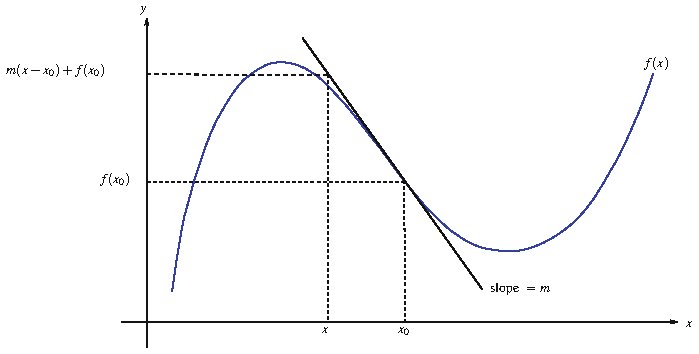
\includegraphics[width=0.943\linewidth]{images/vector/fig-1-12.pdf}
  \caption{函数 $f$ 在点 $x_0$ 处的线性逼近}
  \label{fig:1-12}
\end{figure}

现在我们想考虑上面表达式中 $m(x-x_0)$ 这一部分. 显然 $x-x_0$ 只是某个数，我们把它叫做 $s$. 然后考虑函数 $T:\mathbb{R}\to\mathbb{R}$，其中 $T(s)=ms$. 由于
\[
T(s+t)=m(s+t)=ms+mt=T(s)+T(t)
\qquad\text{且}\qquad
T(cs)=m(cs)=c(ms)=cT(s),
\]
故 $T$ 是一个线性函数，即线性变换. 事实上，$T$ 是在点 $(x_0,f(x_0))$ 处最接近逼近函数 $f$ 的线性函数，见图 \ref{fig:1-12}. 通常，为了简单起见，我们就说 $T$ 是 $f$ 在 $x_0$ 处最接近的线性逼近. 所以对非常接近 $x_0$ 的 $x$ 值，我们有
\[
f(x)\approx\underbrace{m(x-x_0)}_{\text{$f$ 在 $x_0$ 处的线性逼近}}\;+\;\underbrace{f(x_0)}_{\text{把线性逼近上下平移适当量}}.
\]

我们现在要做的是把导数的概念推广到形如 $f:\mathbb{R}^n\to\mathbb{R}^m$ 的函数. 我们假定函数 $f$ 具有形式
\[
f(x_1,x_2,\ldots,x_n)=\bigl(f_1(x_1,x_2,\ldots,x_n),f_2(x_1,x_2,\ldots,x_n),\ldots,f_m(x_1,x_2,\ldots,x_n)\bigr).
\]
我们想找到最接近逼近这个函数 $f:\mathbb{R}^n\to\mathbb{R}^m$ 的线性变换，记为 $Df$，在某个具体的点 $x_0=(x_{10},x_{20},\ldots,x_{n0})\in\mathbb{R}^n$ 处. 若 $f$ 在 $x_0\in\mathbb{R}^n$ 处可微，则存在线性变换 $Df(x_0):\mathbb{R}^n\to\mathbb{R}^m$ 使得
\[
\lim_{x\to x_0}\frac{\|f(x)-f(x_0)-Df(x_0)(x-x_0)\|}{\|x-x_0\|}=0.
\]
这里 $Df(x_0)$ 是一个线性映射，$(x-x_0)$ 是 $\mathbb{R}^n$ 中起点在 $x_0$、终点在 $x$ 的向量，而 $Df(x_0)(x-x_0)$ 是该线性映射作用在向量上的结果，它是 $\mathbb{R}^m$ 中的一个元素. 若 $h$ 是 $\mathbb{R}^n$ 中的向量，有时我们写 $Df(x_0)\cdot h$ 而不是 $Df(x_0)(h)$.

关于 $\|\cdot\|$ 是什么以及为什么需要它，简单说几句. $\|\cdot\|$ 表示称为欧几里得范数的对象，本质上它是绝对值 $|\cdot|$ 的多维版本. 给定向量
\[
v=\begin{bmatrix}x_1\\\vdots\\x_n\end{bmatrix},\qquad\text{则}\qquad
\|v\|=\sqrt{\sum_{i=1}^{n}x_i^2},
\]
这只是向量的长度. 如果你把向量 $v$ 想成点 $(x_0,\ldots,x_n)$，这给出该点到原点的距离. 没有范数，我们定义中的分子和分母都将是 $\mathbb{R}^m$ 中的点或向量（取决于你如何看待它们），而人们不能用一个点或向量除以另一个点或向量. 范数使我们能够简单地相除两个数.

很容易有点糊涂. 记号可能有点歧义. 但通常一点点歧义能带来很大的灵活性，所以这种歧义被容忍，甚至被拥抱. 注意 $Df$、$Df(x)$ 和 $Df(x_0)$ 都用来表示作为函数 $f$ 的逼近的线性变换. 如果我们在泛泛地谈，还没有实际选定具体的基点 $x_0$，那么我们使用 $Df$ 或 $Df(x)$. 如果我们选定了基点 $x_0$，那么我们使用 $Df(x_0)$. 这与说 $f(x)=x^2$ 的导数是 $f'$ 或 $f'(x)$（两者都是 $2x$），而 $f$ 在点 $x_0=3$ 处的导数是 $f'(3)=6$ 非常类似. 此外，画出精确的图像不再可能. 要画出 $f:\mathbb{R}^n\to\mathbb{R}^m$ 的图像，实际上需要画出 $\mathbb{R}^{n+m}$. 我们画的图像当然类似，但必须认识到它实际上是一幅漫画，如图 \ref{fig:1-13} 所示.

\begin{figure}[htbp]
  \centering
  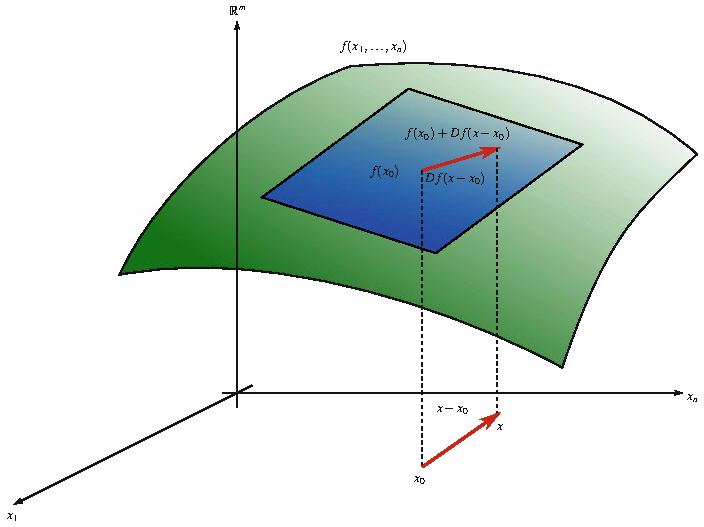
\includegraphics[width=0.960\linewidth]{images/vector/fig-1-13.pdf}
  \caption{函数 $f$ 在点 $x_0$ 处的线性逼近，以三维方式描绘}
  \label{fig:1-13}
\end{figure}

和之前一样，我们有
\[
f(x)\approx\underbrace{Df(x_0)(x-x_0)}_{\text{$f$ 在 $x_0$ 处的线性逼近}}\;+\;\underbrace{f(x_0)}_{\text{把线性逼近适当平移}}.
\]

我们之前看到可以把线性变换写成矩阵，所以我们的目标是把 $Df(x)$ 写成一个矩阵. 使用与之前相同的记号，并假定 $\mathbb{R}^n$ 的基由 $e_j$ 给出、$\mathbb{R}^m$ 的基由 $\tilde{e}_i$ 给出，我们想找到满足下式的 $a_{ij}$：
\[
Df(x)\cdot e_j=\sum_{i=1}^{m}a_{ij}\tilde{e}_i=\begin{bmatrix}a_{1j}\\a_{2j}\\\vdots\\a_{mj}\end{bmatrix}.
\]
换句话说，$Df(x)$ 的第 $j$ 列的第 $i$ 个分量就是 $Df(x)\cdot e_j$ 的第 $i$ 个分量.

为了求 $Df(x)$ 的矩阵表示，回想向量微积分中的结论：给定函数 $f:\mathbb{R}^n\to\mathbb{R}$，我们把 $f$ 关于 $x_j$ 的偏导数定义为
\[
\frac{\partial f}{\partial x_j}=\lim_{h\to0}\frac{f(x_1,\ldots,x_j+h,\ldots,x_n)-f(x_1,\ldots,x_j,\ldots,x_n)}{h}.
\]
当我们给定一个函数
\[
f:\mathbb{R}^n\to\mathbb{R}^m,\qquad
(x_1,\ldots,x_n)\longmapsto\bigl(f_1(x_1,\ldots,x_n),\ldots,f_m(x_1,\ldots,x_n)\bigr)
\]
时，我们当然可以对每个 $f_i$（$1\leq i\leq m$）关于每个 $x_j$（$1\leq j\leq n$）求偏导数，
\[
\frac{\partial f_i}{\partial x_j}=\lim_{h\to0}\frac{f_i(x_1,\ldots,x_j+h,\ldots,x_n)-f_i(x_1,\ldots,x_j,\ldots,x_n)}{h}.
\]
这里有几件事要注意. 首先，$x_j$ 是对应于 $\mathbb{R}^n$ 中基向量 $e_j$ 的坐标，而 $f_i(x_1,\ldots,x_n)\equiv f_i$ 是对应于 $\mathbb{R}^m$ 中基向量 $\tilde{e}_i$ 的坐标. 其次，我们保持 $x_1,\ldots,x_{j-1},x_{j+1},\ldots,x_n$ 固定，只让 $x_j$ 变化. 固定这些变量后的函数 $f_i$ 成为从 $\mathbb{R}$ 到 $\mathbb{R}$ 的函数，因此它最接近的线性逼近只是一个表示斜率的数，记为 $a_{ij}$. 于是我们有
\[
\frac{\partial f_i}{\partial x_j}=a_{ij}.
\]

考虑我们对 $Df(x_0)$ 的定义，即它是满足
\[
\lim_{x\to x_0}\frac{\|f(x)-f(x_0)-Df(x_0)(x-x_0)\|}{\|x-x_0\|}=0
\]
的线性变换，其中 $Df(x_0)(x-x_0)$ 是 $\mathbb{R}^m$ 中的列向量，而 $x-x_0$ 是 $\mathbb{R}^n$ 中的向量.

为了求 $Df(x_0)$ 的 $a_{ij}$，我们需要求 $Df(x_0)\cdot e_j$ 的第 $i$ 个元素. 令
\[
x=\begin{bmatrix}x_{10}\\x_{20}\\\vdots\\x_{n0}\end{bmatrix}+h\begin{bmatrix}0\\\vdots\\1\\\vdots\\0\end{bmatrix}=x_0+he_j,
\]
我们可以把上面的式子写为
\begin{align*}
\lim_{x\to x_0}\frac{\|f(x)-f(x_0)-Df(x_0)(he_j)\|}{\|he_j\|}&=0\\
\Rightarrow\quad\lim_{h\to0}\frac{\left\|\begin{aligned}
&f(x_{10},\ldots,x_{i0}+h,\ldots,x_{n0})\\
&\quad-f(x_{10},\ldots,x_{i0},\ldots,x_{n0})\\
&\quad-hDf(x_0)\cdot e_j
\end{aligned}\right\|}{|h|}&=0.
\end{align*}
这个表达式的分子是 $\mathbb{R}^m$ 中的一个向量，其第 $i$ 个分量通过看函数 $f$ 定义中的 $f_i$ 得到. 于是 $Df(x_0)$ 的第 $j$ 列的第 $i$ 个分量由下式给出：
\begin{align*}
\lim_{h\to0}\frac{\left|\begin{aligned}
&f_i(x_{10},\ldots,x_{i0}+h,\ldots,x_{n0})\\
&\quad-f_i(x_{10},\ldots,x_{i0},\ldots,x_{n0})\\
&\quad-ha_{ij}
\end{aligned}\right|}{|h|}&=0\\
\Rightarrow\quad a_{ij}&=\lim_{h\to0}\frac{\begin{aligned}
f_i(x_{10},\ldots,x_{i0}+h,\ldots,x_{n0})\\
-f_i(x_{10},\ldots,x_{i0},\ldots,x_{n0})
\end{aligned}}{h}
\end{align*}
但这恰恰就是 $\frac{\partial f_i}{\partial x_j}$. 因此，$Df(x)$ 的矩阵表示由一个称为 $f$ 的 \newterm{jacobian-matrix}{Jacobian 矩阵}{Jacobian matrix} 的矩阵给出：
\[
Df(x)=\begin{bmatrix}
\frac{\partial f_1}{\partial x_1}&\frac{\partial f_1}{\partial x_2}&\cdots&\frac{\partial f_1}{\partial x_n}\\[2mm]
\frac{\partial f_2}{\partial x_1}&\frac{\partial f_2}{\partial x_2}&\cdots&\frac{\partial f_2}{\partial x_n}\\
\vdots&\vdots&\ddots&\vdots\\
\frac{\partial f_m}{\partial x_1}&\frac{\partial f_m}{\partial x_2}&\cdots&\frac{\partial f_m}{\partial x_n}
\end{bmatrix}
=\left(\frac{\partial f_i}{\partial x_j}\right)_{\substack{i=\text{行}\\j=\text{列}}}.
\]

\section{小结、参考文献与问题}

\subsection{小结}

每章的小结包含该章所涵盖的最重要的概念与公式，以及必要的结束语. 小结一节的用意是既作为快速参考，也作为章节复习.

向量空间是一个集合 $V$，配备加法 $+$ 与标量乘法 $\cdot$、加法单位元 $0$，以及一个``取负运算''，并满足以下八条公理. 给定向量空间元素 $u,v,w\in V$ 和标量 $c,d\in\mathbb{R}$，这八条公理是
\begin{enumerate}
  \item $v+w=w+v$
  \item $(u+v)+w=u+(v+w)$
  \item $v+0=v=0+v$
  \item $v+(-v)=0$
  \item $1\cdot v=v$
  \item $c\cdot(d\cdot v)=(c\cdot d)\cdot v$
  \item $c\cdot(v+w)=c\cdot v+c\cdot w$
  \item $(c+d)\cdot v=c\cdot v+d\cdot v
  $
\end{enumerate}
向量空间最重要的例子是 $\mathbb{R}^n$. $\mathbb{R}^n$ 的元素写成列向量. 向量空间 $V$ 的基是满足线性无关且张成该向量空间的元素集 $\{v_1,\ldots,v_n\}$. 线性泛函 $T:\mathbb{R}^n\to\mathbb{R}$ 是具有以下两条性质的映射：
\begin{enumerate}
  \item $T(v+w)=T(v)+T(w)$
  \item $T(c\cdot v)=c\cdot T(v)$
\end{enumerate}
其中 $v,w\in\mathbb{R}^n$，$c\in\mathbb{R}$. $\mathbb{R}^n$ 的对偶空间是 $\mathbb{R}^n$ 上所有线性泛函的集合，即所有满足这两条性质的映射 $T:\mathbb{R}^n\to\mathbb{R}$. $\mathbb{R}^n$ 的对偶空间记为 $(\mathbb{R}^n)^*$. 向量空间 $V$ 的任意一组基都诱导出 $V^*$ 的一组对偶基.

利用我们期望平行六面体体积如何表现的三条性质，我们发现体积天然带有符号. 此外，利用这些性质我们能够推导出矩阵行列式的公式，它求以矩阵的列为边的平行六面体的有向体积.

\begin{center}
\textbf{矩阵的行列式公式：}
\end{center}
\[
\begin{vmatrix}a_{11}&a_{12}&\cdots&a_{1n}\\a_{21}&a_{22}&\cdots&a_{2n}\\\vdots&\vdots&\ddots&\vdots\\a_{n1}&a_{n2}&\cdots&a_{nn}\end{vmatrix}
=\sum_{\sigma\in S_n}\mathrm{sgn}(\sigma)\prod_{i=1}^{n}a_{\sigma(i)i}.
\]

最后，给定由 $f=(f_1,\ldots,f_m)$ 定义的函数 $f:\mathbb{R}^n\to\mathbb{R}^m$，该函数的导数 $Df$ 是由 Jacobian 矩阵给出的线性变换
\[
Df(x)=\begin{bmatrix}
\frac{\partial f_1}{\partial x_1}&\frac{\partial f_1}{\partial x_2}&\cdots&\frac{\partial f_1}{\partial x_n}\\[2mm]
\frac{\partial f_2}{\partial x_1}&\frac{\partial f_2}{\partial x_2}&\cdots&\frac{\partial f_2}{\partial x_n}\\
\vdots&\vdots&\ddots&\vdots\\
\frac{\partial f_m}{\partial x_1}&\frac{\partial f_m}{\partial x_2}&\cdots&\frac{\partial f_m}{\partial x_n}
\end{bmatrix}
=\left(\frac{\partial f_i}{\partial x_j}\right)_{\substack{i=\text{行}\\j=\text{列}}}.
\]

\subsection{参考文献与进一步阅读}

本章所呈现的材料都是相当标准的，不过呈现材料所采用的具体方式与本书其余部分的要求一致. 关于线性代数的书不胜枚举，但 Friedberg、Insel 与 Spence 的著作~\cite{ref22} 是一本很好的参考书. 行列式与平行六面体体积的关系也是标准材料，但这里的介绍大体上遵循了一份很好的匿名且未注明日期的关于行列式的讲解~\cite{ref02}. 另见 Abraham、Marsden 与 Ratiu 的著作~\cite{ref01}. 就多元微积分而言，Stewart 的教科书~\cite{ref43} 是一本标准教材. 对于多元微积分稍许更详细的数学介绍，Marsden 与 Hoffman 的书~\cite{ref31} 非常好. 特别是，Marsden 倾向于使用一些出色的记号，本书大部分内容都使用了这些记号.

\subsection{问题}

\begin{question}\label{q:1-18}
令 $V=\{(x_1,x_2)\mid x_1,x_2\in\mathbb{R}\}$. 也就是说，$V$ 是实数有序对的集合. 若 $(a_1,a_2),(b_1,b_2)\in V$ 且 $c\in\mathbb{R}$ 是标量，定义
\[
(a_1,a_2)+(b_1,b_2)=(a_1+b_1,a_2b_2),\qquad c(a_1,a_2)=(ca_1,a_2).
\]
在这些运算下 $V$ 是向量空间吗？
\end{question}

\begin{question}\label{q:1-19}
令 $V=\{(x_1,x_2)\mid x_1,x_2\in\mathbb{R}\}$. 若 $(a_1,a_2),(b_1,b_2)\in V$ 且 $c\in\mathbb{R}$ 是标量，定义
\[
(a_1,a_2)+(b_1,b_2)=(a_1+b_1,a_2+b_2),\qquad c(a_1,a_2)=(a_1,0).
\]
在这些运算下 $V$ 是向量空间吗？
\end{question}

\begin{question}\label{q:1-20}
令 $V=\{(x_1,x_2)\mid x_1,x_2\in\mathbb{R}\}$. 若 $(a_1,a_2),(b_1,b_2)\in V$ 且 $c\in\mathbb{R}$ 是标量，定义
\[
(a_1,a_2)+(b_1,b_2)=(a_1+3b_1,a_2+5b_2),\qquad c(a_1,a_2)=(ca_1,ca_2).
\]
在这些运算下 $V$ 是向量空间吗？
\end{question}

\begin{question}\label{q:1-21}
令 $V=\{(x_1,x_2)\mid x_1,x_2\in\mathbb{R}\}$. 若 $(a_1,a_2),(b_1,b_2)\in V$ 且 $c\in\mathbb{R}$ 是标量，定义
\[
(a_1,a_2)+(b_1,b_2)=(a_1+b_1,a_2+b_2),\qquad
c(a_1,a_2)=\begin{cases}(0,0)&c=0\\\left(ca_1,\frac{a_2}{c}\right)&c\neq0.\end{cases}
\]
在这些运算下 $V$ 是向量空间吗？
\end{question}

\begin{question}\label{q:1-22}
设 $V$、$W$ 是向量空间，令 $Z=\{(v,w)\mid v\in V,\,w\in W\}$. 若 $(v_1,w_1)$、$(v_2,w_2)\in Z$，且 $c\in\mathbb{R}$ 是标量，定义
\[
(v_1,w_1)+(v_2,w_2)=(v_1+v_2,w_1+w_2),
\]
且
\[
c(v_1,w_1)=(cv_1,cw_1).
\]
证明 $Z$ 是向量空间.
\end{question}

\begin{question}\label{q:1-23}
考虑向量
\[
v_1=\begin{bmatrix}1\\3\\-4\\2\end{bmatrix},\qquad
v_2=\begin{bmatrix}1\\1\\-2\\0\end{bmatrix},\qquad
v_3=\begin{bmatrix}1\\-3\\2\\-4\end{bmatrix},\qquad
v_4=\begin{bmatrix}-2\\0\\2\\0\end{bmatrix}.
\]
证明这些向量线性相关. 也就是说，找到不全为零的标量 $c_1,c_2,c_3,c_4$，使得
\[
c_1v_1+c_2v_2+c_3v_3+c_4v_4=\begin{bmatrix}0\\0\\0\\0\end{bmatrix}.
\]
\end{question}

\begin{question}\label{q:1-24}
考虑向量
\[
v_1=\begin{bmatrix}1\\0\\0\\-1\end{bmatrix},\qquad
v_2=\begin{bmatrix}0\\1\\0\\-1\end{bmatrix},\qquad
v_3=\begin{bmatrix}0\\0\\1\\-1\end{bmatrix},\qquad
v_4=\begin{bmatrix}0\\0\\0\\1\end{bmatrix}.
\]
证明这些向量线性无关. 为此证明：使得
\[
c_1v_1+c_2v_2+c_3v_3+c_4v_4=\begin{bmatrix}0\\0\\0\\0\end{bmatrix}
\]
成立的唯一线性组合是其中所有标量 $c_1,c_2,c_3,c_4$ 都为零的那一个.
\end{question}

\begin{question}\label{q:1-25}
给出 $\mathbb{R}^3$ 中三个线性相关向量的集合，使得其中任何一个向量都不是其余向量中另一个的倍数.
\end{question}

\begin{question}\label{q:1-26}
给出 $\mathbb{R}^4$ 中四个线性相关向量的集合，使得其中任何一个向量都不是其余向量中另一个的倍数.
\end{question}

\begin{question}\label{q:1-27}
向量 $v_1=\begin{bmatrix}1\\1\end{bmatrix}$、$v_2=\begin{bmatrix}1\\-2\end{bmatrix}$ 张成 $\mathbb{R}^2$ 吗？也就是说，对任意向量 $v\in\mathbb{R}^2$，能否找到标量 $c_1,c_2$ 使得 $c_1v_1+c_2v_2=v$？
\end{question}

\begin{question}\label{q:1-28}
向量 $v_1=\begin{bmatrix}1\\1\\0\end{bmatrix}$、$v_2=\begin{bmatrix}0\\1\\1\end{bmatrix}$、$v_3=\begin{bmatrix}1\\0\\1\end{bmatrix}$ 张成 $\mathbb{R}^3$ 吗？也就是说，对任意向量 $v\in\mathbb{R}^3$，能否找到标量 $c_1,c_2,c_3$ 使得 $c_1v_1+c_2v_2+c_3v_3=v$？
\end{question}

\begin{question}\label{q:1-29}
向量 $v_1=\begin{bmatrix}4\\2\\0\end{bmatrix}$、$v_2=\begin{bmatrix}0\\1\\1\end{bmatrix}$、$v_3=\begin{bmatrix}2\\2\\1\end{bmatrix}$ 张成 $\mathbb{R}^3$ 吗？也就是说，对任意向量 $v\in\mathbb{R}^3$，能否找到标量 $c_1,c_2,c_3$ 使得 $c_1v_1+c_2v_2+c_3v_3=v$？
\end{question}

\begin{question}\label{q:1-30}
若 $T:V\to W$ 是线性变换，证明 $T(\mathbf{0}_V)=\mathbf{0}_W$，其中 $\mathbf{0}_V$ 是 $V$ 中的零向量，$\mathbf{0}_W$ 是 $W$ 中的零向量.
\end{question}

\begin{question}\label{q:1-31}
若 $T:V\to W$ 是线性变换，证明 $T(cx+y)=cT(x)+T(y)$.
\end{question}

\begin{question}\label{q:1-32}
若 $T:V\to W$ 是线性变换，证明
\[
T\left(\sum_{i=1}^{n}a_iv_i\right)=\sum_{i=1}^{n}c_iT(v_i).
\]
\end{question}

\begin{question}\label{q:1-33}
定义 $T:\mathbb{R}^2\to\mathbb{R}^2$ 为
\[
T\binom{x_1}{x_2}=\binom{2x_1+x_2}{x_1}.
\]
$T$ 是线性变换吗？如果是，求 $T$ 的矩阵表示.
\end{question}

\begin{question}\label{q:1-34}
对任意角度 $\theta$，定义 $T_\theta:\mathbb{R}^2\to\mathbb{R}^2$ 为
\[
T_\theta\binom{x_1}{x_2}=\binom{x_1\cos\theta-x_2\sin\theta}{x_1\sin\theta+x_2\cos\theta}.
\]
证明 $T_\theta$ 是线性变换. 变换 $T_\theta$ 称为绕 $\theta$ 角的旋转. 求 $T_\theta$ 的矩阵表示.
\end{question}

\begin{question}\label{q:1-35}
定义 $T:\mathbb{R}^2\to\mathbb{R}^2$ 为
\[
T\binom{x_1}{x_2}=\binom{x_1}{-x_2}.
\]
证明 $T$ 是线性变换. 变换 $T$ 称为关于 $x$ 轴的反射. 求 $T$ 的矩阵表示.
\end{question}

\begin{question}\label{q:1-36}
令
\[
\left\{\begin{bmatrix}2\\1\end{bmatrix},\begin{bmatrix}3\\1\end{bmatrix}\right\}
\]
为 $\mathbb{R}^2$ 的一组基. 求对偶基. 也就是说，求与这组基对偶的 $(\mathbb{R}^2)^*$ 的基.
\end{question}

\begin{question}\label{q:1-37}
利用行列式公式，求常数 $C$ 使得
\[
\begin{vmatrix}2a_1&2a_2&2a_3\\3b_1+4c_1&3b_2+4c_2&3b_3+4c_3\\5c_1&5c_2&5c_3\end{vmatrix}
=C\begin{vmatrix}a_1&a_2&a_3\\b_1&b_2&b_3\\c_1&c_2&c_3\end{vmatrix}.
\]
\end{question}

\begin{question}\label{q:1-38}
令
\[
\left\{\begin{bmatrix}1\\0\\1\end{bmatrix},\begin{bmatrix}1\\2\\1\end{bmatrix},\begin{bmatrix}0\\0\\1\end{bmatrix}\right\}
\]
为 $\mathbb{R}^3$ 的一组基. 求对偶基.
\end{question}

\begin{question}\label{q:1-39}
利用行列式公式，求常数 $C$ 使得
\[
\begin{vmatrix}3a_1&3a_2&3a_3\\3b_1&3b_2&3b_3\\3c_1&3c_2&3c_3\end{vmatrix}
=C\begin{vmatrix}a_1&a_2&a_3\\b_1&b_2&b_3\\c_1&c_2&c_3\end{vmatrix}.
\]
\end{question}

\begin{question}\label{q:1-40}
求下列矩阵的行列式的值：
\[
\begin{bmatrix}2&-6\\-2&5\end{bmatrix},\qquad
\begin{bmatrix}3&0&5\\-2&-1&4\\7&6&0\end{bmatrix},\qquad
\begin{bmatrix}0&1&3\\-1&0&-3\\2&3&0\end{bmatrix}.
\]
\end{question}

\begin{question}\label{q:1-41}
求下列函数的 Jacobian 矩阵：
\begin{enumerate}
  \item[(a)] $f(x,y)=xy$
  \item[(b)] $f(x,y)=\sin(x^3+y^2)$
  \item[(c)] $f(x,y,z)=x^5+y^4$
  \item[(d)] $f(x,y)=\bigl(\sin(x\sin(y)),(x+y)^2\bigr)$
  \item[(e)] $f(x,y)=\bigl(\cos(xy),\sin(xy),x^2y^2\bigr)$
  \item[(f)] $f(x,y,z)=\bigl(z^{xy},x^2,\tan(xyz)\bigr)$
\end{enumerate}
\end{question}
